\documentclass[12pt,a4paper,notitlepage]{article}
\usepackage[utf8]{inputenc}
\usepackage[english]{babel}
\usepackage[T1]{fontenc}
\usepackage[backend=biber,
			style=authoryear-comp,
			isbn=false,
			doi=false,
			bibstyle=authoryear,
			natbib,
			]{biblatex}
\usepackage{eurosym}
\usepackage{enumitem}
\usepackage{url}
\usepackage{blindtext}
\usepackage{hyperref}
\usepackage{breakurl}
\usepackage{amsmath}
\usepackage{titling}
\usepackage{amsfonts}
\usepackage{amssymb}
\usepackage{pgfplots}
\usepackage{caption}
\usepackage{subcaption}
\usepackage{graphicx}
\usepackage{dcolumn}
\usepackage{tikz-3dplot}
\usepackage{subcaption}
\usepackage{float}
\usepackage{adjustbox}
\usepackage{multirow,rotating}
\usepackage[autostyle]{csquotes}
\usepackage[toc,page]{appendix}
\usepackage{lscape}
\usepackage{todonotes}
\usepackage{booktabs}
\usepackage{multirow}
\usepackage{bm}
\usepackage{eurosym}
\usepackage{pdflscape}
\usepackage{geometry}
\geometry{a4paper,left=30mm,right=20mm, top=2cm, bottom=2cm} 

\addbibresource{Textmining.bib}

\title{Topic and tone of political news articles in German online media.}
\date{\today}
\author{Franziska Löw}

\begin{document}
\begin{titlepage}
	\maketitle
	\begin{abstract}
		The aim of this paper is to investigate whether the political reporting of different content providers distinguishes itself and whether this reporting has an influence on the opinion-forming process of the voters. 
		
		\textbf{Keywords} Structural Topic Model, Sentiment Analysis, Unsupervised Machine Learning, Text Mining

	\end{abstract}

\end{titlepage}

\tableofcontents

\section{Introduction}
% Paper von Ralf, Melissa, Tobias zitieren. 

The discussion about the influence of digital media on the political opinion-forming process has gained momentum since the presidential elections in the USA in October 2016 at the latest. Overall, the importance of the Internet as a source of information for political topics has been very strong in recent years. According to a study on the media coverage of the German-speaking population, nearly 40\% of respondents used the internet at least once a week in 2017 to inform themselves about the current news compared to 34\% in 2016 \citep{vuma_arbeitsgemeinschaft_verbrauchs-_und_medienanalyse_verbrauchs-_2017}.

The pluralism nor only of online media, but of media in general is an essential principle of democratic societies. For the process of forming opinions, information conveyed by the media, in particular the mass media of journalism, plays a decisive role. An important question is therefore whether there are convergence tendencies within the mass media - that is, whether popular media tend to report on certain political topics in the same or similar ways and whether this reporting has an influence on the opinion-forming process of the voters. With the purpose of examining the media pluralism in the market for German-language online news, this paper analyzes German online news articles about domestic politics. German federal elections took place on 24th of September 2017 and the formation of the government has taken up a period of about five month. The articles considered here dated from 01.06.2017 to 01.03.2018 and thus inform their readers both about the election promises of the parties (before the election) and about the coalition talks (after the election). They therefore make an important contribution to the public's opinion-forming process. The empirical strategy follows a novel approach combining "the two Ts": Topic and Tone \citep{hansen_shocking_2016}. This means that the topics discussed in the articles are identified first (topic), followed by an analysis of how they are discussed with the various news websites (tone). The final step is to check whether the tonality of reporting is reflected in the survey results on voting preferences calculating the cross correlation coefficients. More precisely, the research strategy is as follows:

\begin{enumerate}
	\item\label{item_1} \textbf{Discovering Topics (Section \ref{subsection_topic})} To discover the latent topics in the corpus, the structural topic modeling (STM) developed by \citet{roberts_model_2016} is applied. The STM is an unsupervised machine learning approach that models topics as multinomial distributions of words and documents (as a synonym for news articles) as multinomial distributions of topics, allowing to incorporate external variables that effect both, topical content and topical prevalence. I estimate a model, where the news website is included as a control for both the topical content and the topical prevalence. The result of the generative process of STM are two posterior distributions: One for the topic prevalence in an article and one for the content of a topic. The latter is used to label the topics according to an event or issue discussed in the media. The topic prevalence of an article (or the posterior distribution) is used to assign a topic to each news article. 
	\item\label{item_2} \textbf{Measuring Tone (Section \ref{subsection_tone})} After assigning a topic to each article, a dictionary-based sentiment analysis is conducted to estimate how topics are discussed differently by different news websites. The idea of a sentiment analysis is to determine the attitude of a writer toward the overall tonality of a document. To conduct such an analysis, a lists of words (dictionary) associated with a given emotion, such as negativity is pre-defined by the analyst. The document is then deconstructed into individual words and the frequencies of words contained in a given dictionary are calculated.
	\item\label{item_3} \textbf{Comparing with polls} In order to check whether the transmitted content from the online media is reflected in the voting preferences, the relationship between monthly average of the emotional value of individual topics from \ref{item_2} and the survey value of a specific party is estimated using the cross correlation function (CCF).
\end{enumerate}

Approach \ref{item_1} has been used in \citet{roberts_model_2016}, among others, to examine differences in the content of eastern and western news providers regarding "the rise of China". However, I extend the analysis by comparing the sentiment score for a given topic an news provider, to identify which topics are discussed similar or differently (\ref{item_2}). \citet{hansen_shocking_2016} applied a similar approach to a dataset of 142 FOMC (Federal Open Market Committee) decision statements to measure the effect of those statements on macroeconomic variables. An additional extension is the comparison with current election poll values (\ref{item_3}). 

The remaining course of the paper is as follows: The following Section \ref{ch_elections} gives an overview about political trends in the past six month (June 2017 to March 2018). The data used to conduct the model is described in Section \ref{ch_data}. Section \ref{ch_model} explains the generative process of the structural topic model as well as the selected parameters to run the model. The empirical analysis containing the above mentioned steps is conducted in Section \ref{ch_empirical}. 
 
% -------------------------
% Background Bundestagswahl
% -------------------------
\section{Background on the federal election in Germany (2017)}\label{ch_elections}

The articles analyzed in this paper cover a period from June 1, 2017 to March 1, 2018 and thus cover both the most important election campaign topics for the Bundestag elections on September 24, 2017 and the process of forming a government that lasted until February 2018. After four years in a grand coalition with the Social Democrats (SPD), German Chancellor Angela Merkel, member of the Conservative Party (CDU/CSU, also known as Union), ran for re-election. The SPD nominated Martin Schulz as candidate for chancellor. 

On the right side of the political spectrum, AfD (alternative for Germany) managed to be elected to the German Bundestag for the first time in 2017. The political debate about the high refugee numbers of the past years brought the AfD a political upswing by taking up the dissatisfaction of parts of the population and using it to raise its own profile. Leading party members of the AfD as well as party supporters repeatedly accused the mass media in the course of the reporting on the federal elections to report unilaterally and to present the AfD intentionally badly.

After the election, the formation of a government was difficult due to the large number of parties elected to the Bundestag and the considerable loss of votes by the major parties CDU/CSU and SPD. Since all parties rejected a coalition with the AfD, numerically only two coalitions with an absolute parliamentary majority were possible: a grand coalition ("GroKo" - from the German word Große Koalition) of CDU/CSU and SPD, and a Jamaica coalition (coalition of CDU/CSU, FDP (economic liberal party) and B90/Die Grünen (Bündnis 90/Die Grünen, green party)). The grand coalition was initially rejected by the SPD. The four-week exploratory talks on the possible formation of a Jamaica coalition officially failed on 19 November 2017 after the FDP announced its withdrawal from the negotiations. FDP party leader Christian Lindner said that there had been no trust between the parties during the negotiations. The main points of contention were climate and refugee policy. CDU and CSU regretted this result, while B90/Die Grünen sharply criticized the withdrawal of the Liberals. The then Green leader Cem Özdemir accused the FDP of lacking the will to reach an agreement.

After the failure of the Jamaica coalition, a possible re-election or a minority government as alternatives were discussed in the media before the SPD decided to hold coalition talks with the CDU/CSU. This led to great resistance from the party base, which called for a party-internal vote on a grand coalition. After the party members voted in favor of the grand coalition, a government was formed 171 days after the federal elections. 

Figure \ref{fig_polls} shows that support for the two major popular parties has been declining in recent months since August 2017, with the CDU/CSU again showing positive survey results since November. However, the value of the SPD has been falling since March 2017. At the same time, the AfD in particular has been recording increasingly positive survey results since June 2017. Section \ref{ch_correlation} examines whether there is a correlation between the survey results and the way the parties are reported in the media. 

\begin{figure}[H]
\begin{center}
	\caption{Election Polls}
	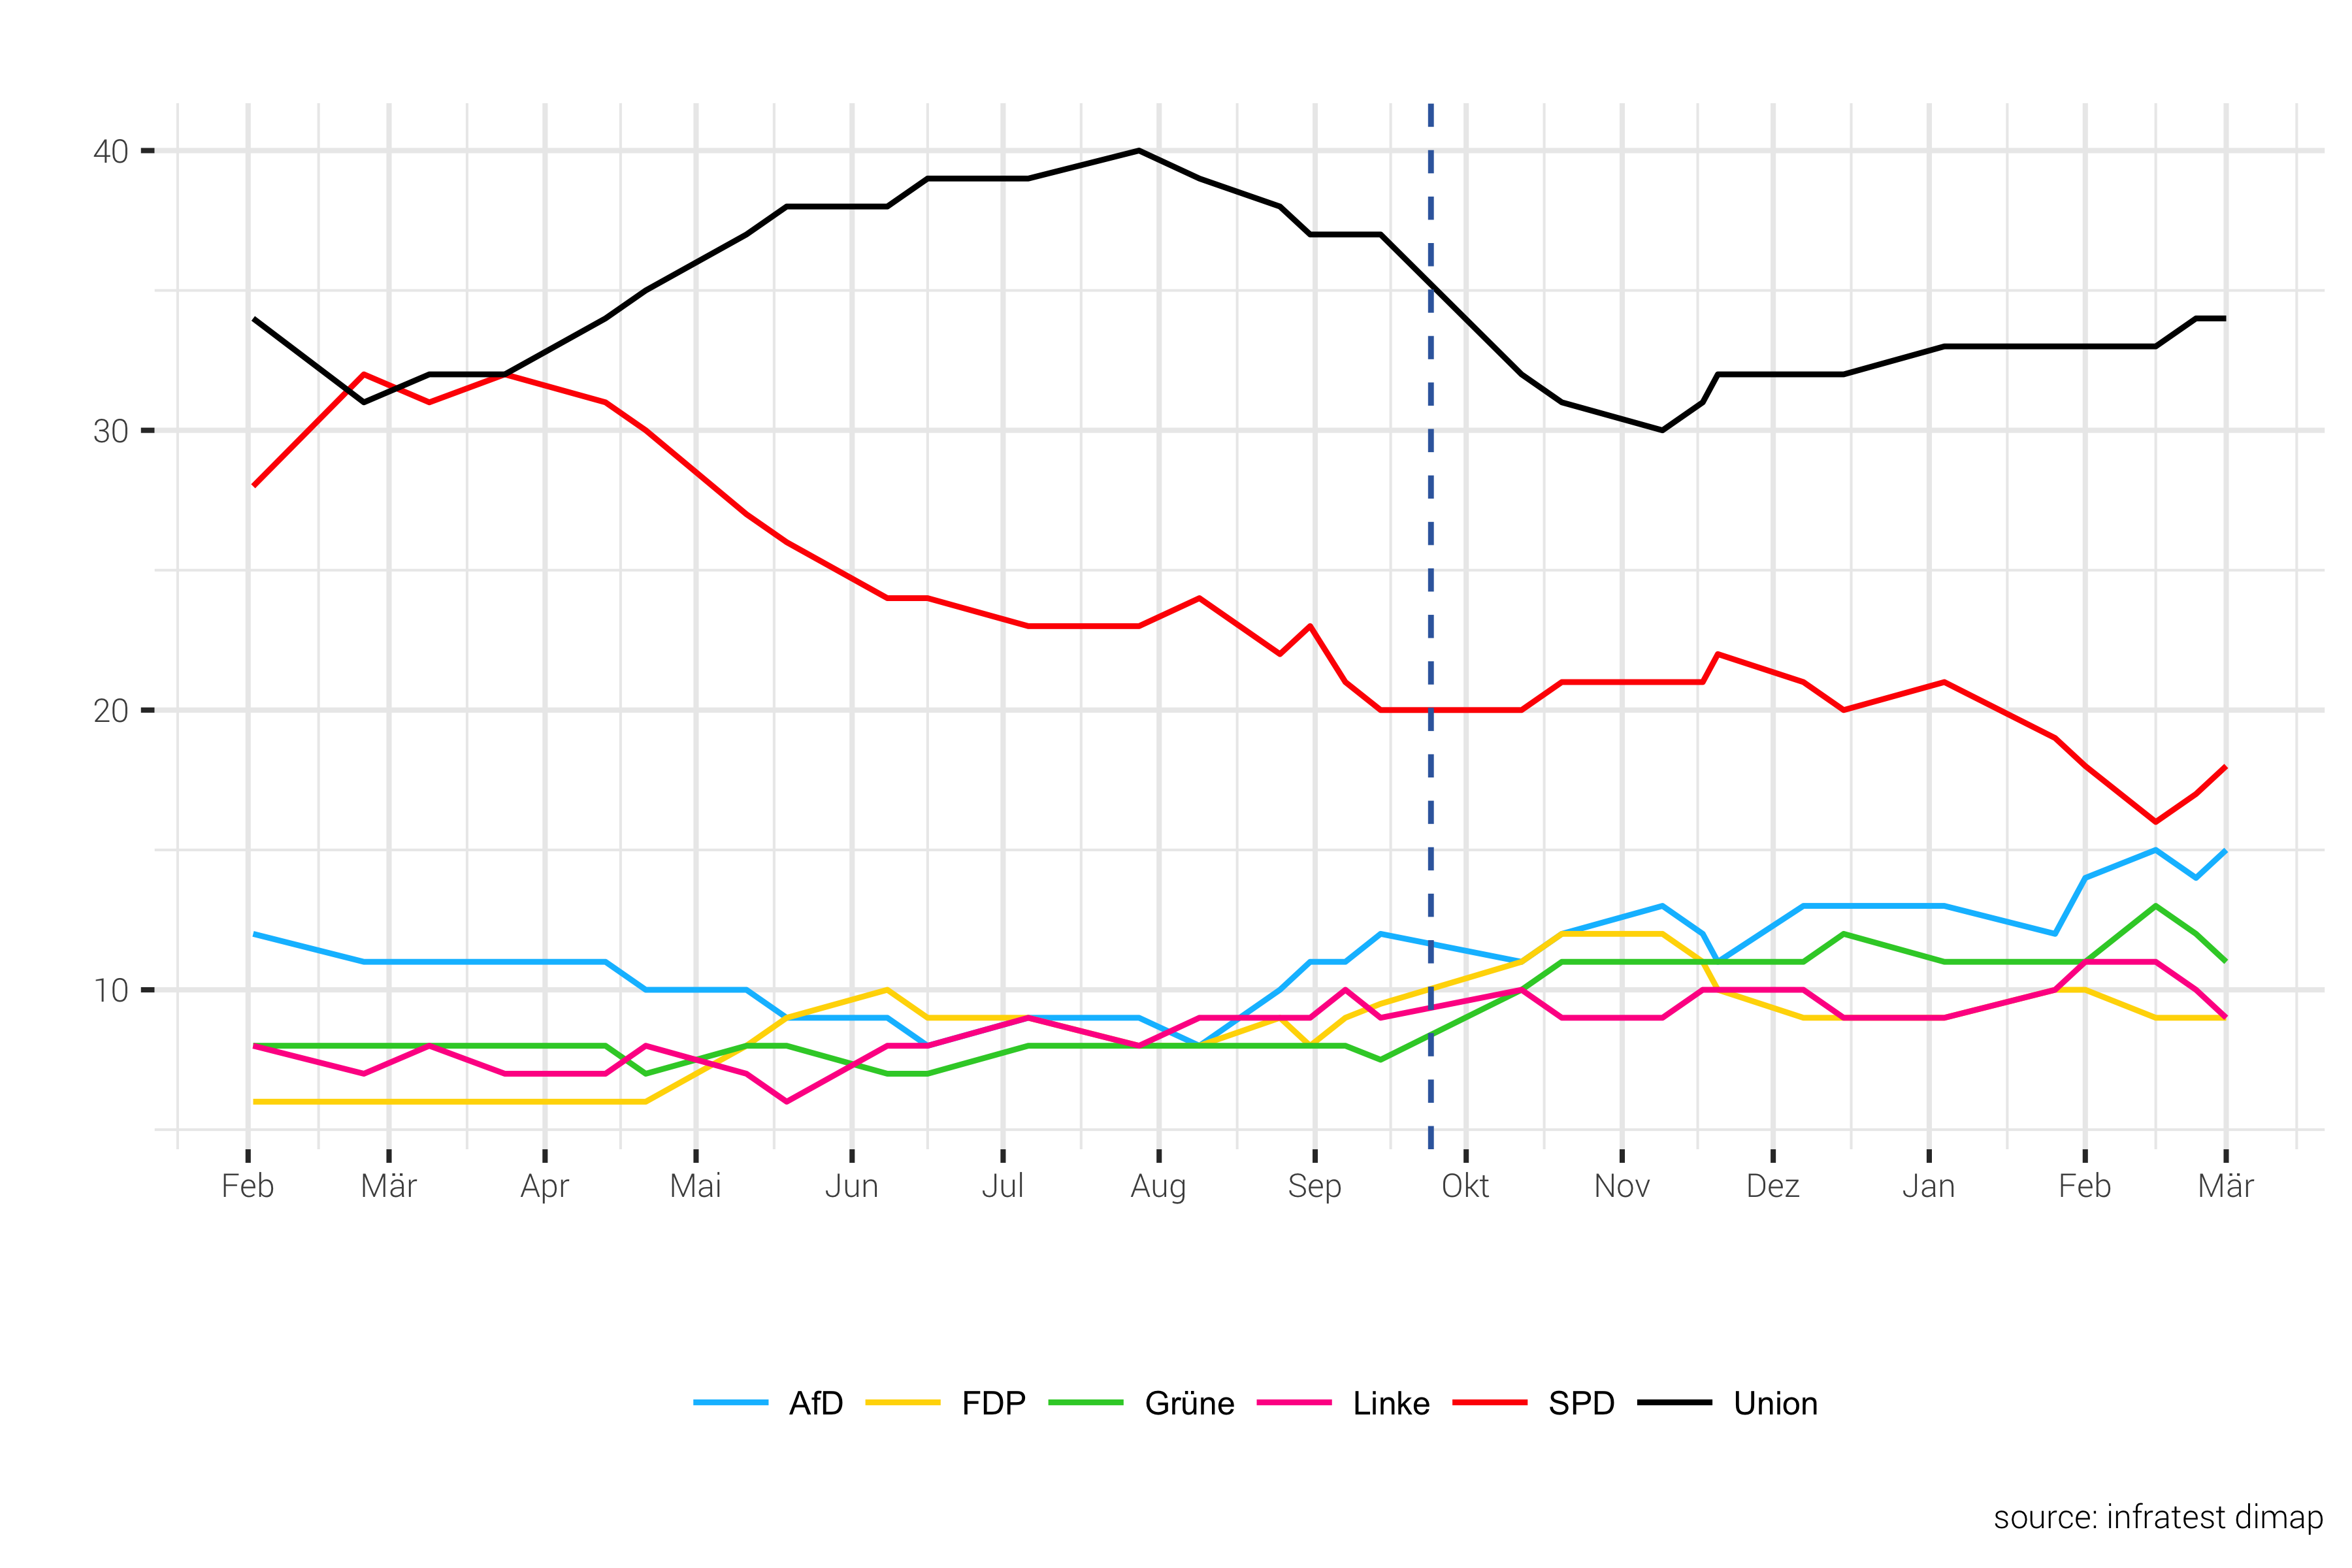
\includegraphics[width=0.8\textwidth]{../figs/polls.png}
	\label{fig_polls}
	\end{center}
\end{figure}

% -----
% Data
% -----
\section{Dataset and data preparation}\label{ch_data}

I conduct the estimation on a sample of 14,937 online news articles from seven german news provider about domestic politics\footnote{Bild.de, DIE WELT, FOCUS ONLINE, SPIEGEL ONLINE, stern.de, ZEIT ONLINE, Tagesschau.de}.  The articles are dated from 01.06.2017 to 01.03.2018. I first extract all online articles using the the Webhose.io API.\footnote{For more information see https://docs.webhose.io/v1.0/docs/getting-started. The scraping code was written in Python and can be made available on request.} Then all articles from the section "domestic policy" are filtered by using the URL of an article. Overall, the selected news providers are among the top ten German online news providers - in terms of unique user\footnote{The term unique user refers to a number of different visitors to a website within a certain period of time. Multiple visits from the same user are only considered once.} - in the period under review, with only Tagesschau.de belonging to the public media. The reason for this is that the content structure of Tagesschau.de is most similar to that of the private providers. ZDF.de offers predominantly video content and DLF (Deutschlandfunk) website mainly offers audio content in the form of interviews, which makes it hard to include it in the model. 

 Figure \ref{fig_distr1} shows the distribution of the number of articles by date. There is a high peak around the federal elections on September, 24th and another one shortly after the failure of the Jamaica coalition talks on November, 19th (indicated by the red dotted lines). Figure \ref{fig_distr2} shows, that DIE WELT published most articles on domestic policy, followed by stern.de and FOCUS ONLINE.  

\begin{figure}[H]
	\caption{Article distribution...}
	\begin{center}
		\begin{subfigure}[normla]{0.49\textwidth}
			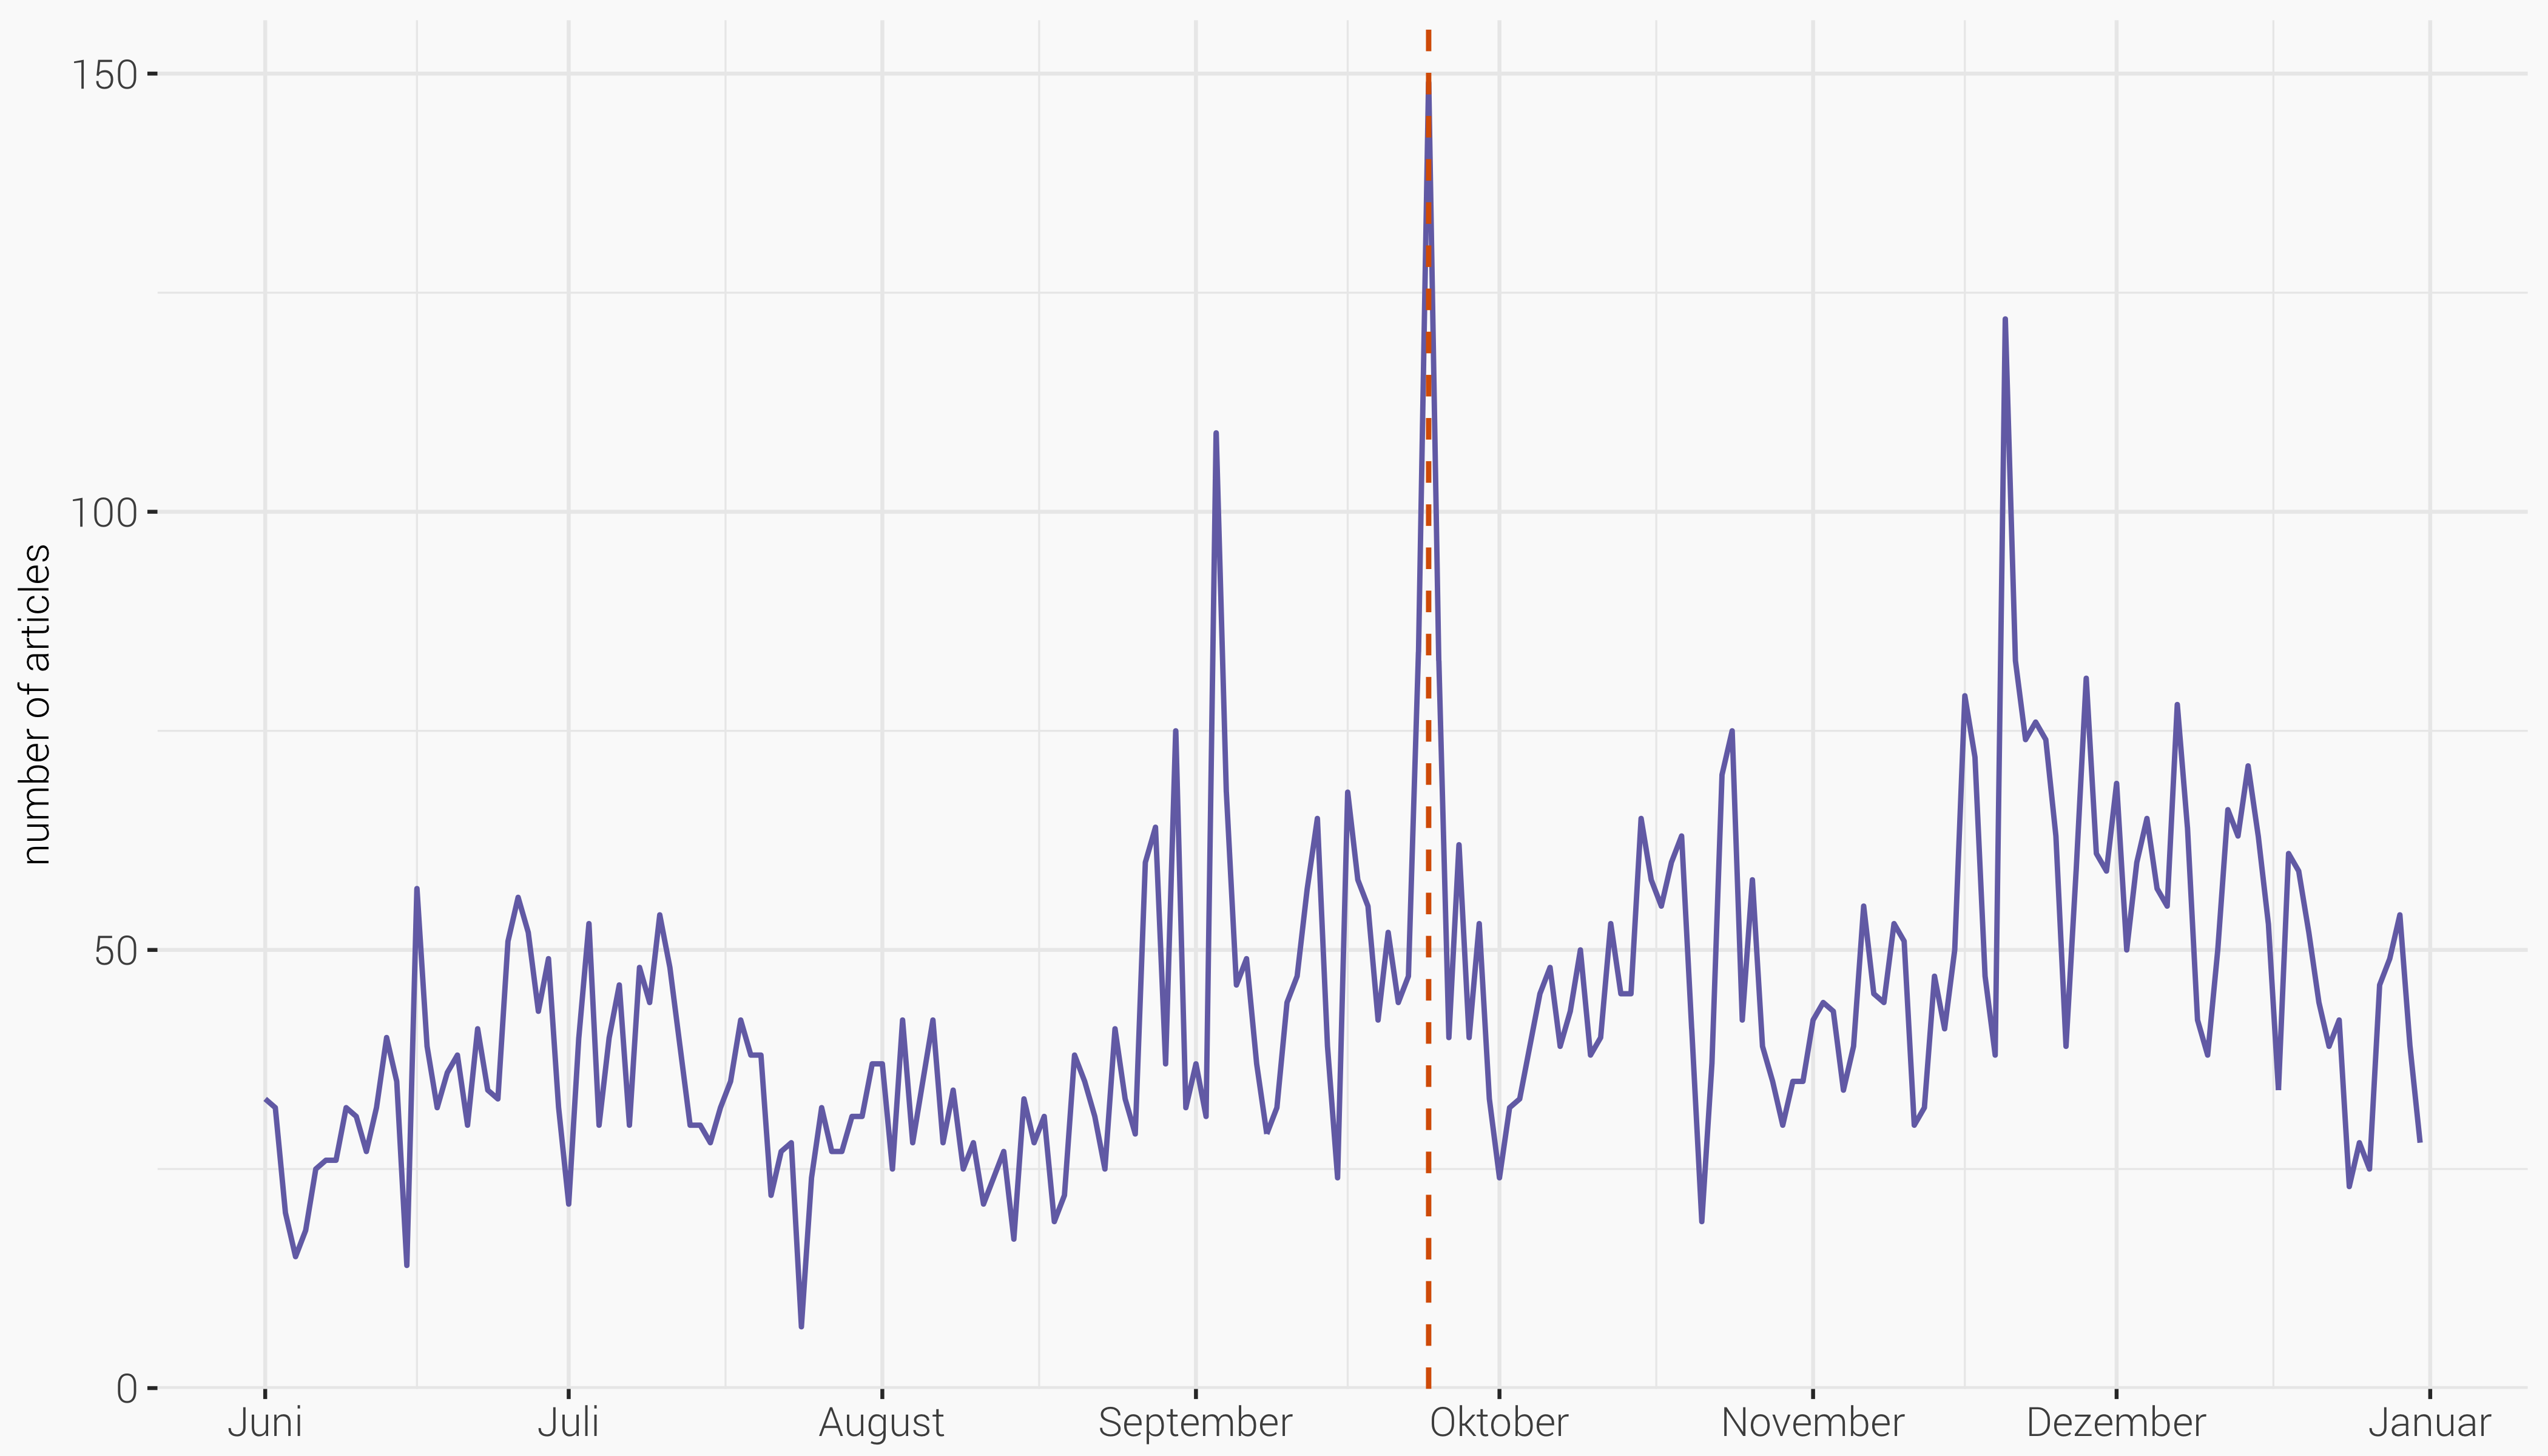
\includegraphics[width=\textwidth]{../figs/timeline.png}
			\caption{...by date}
			\label{fig_distr1}
		\end{subfigure}
		\begin{subfigure}[normla]{0.49\textwidth}
			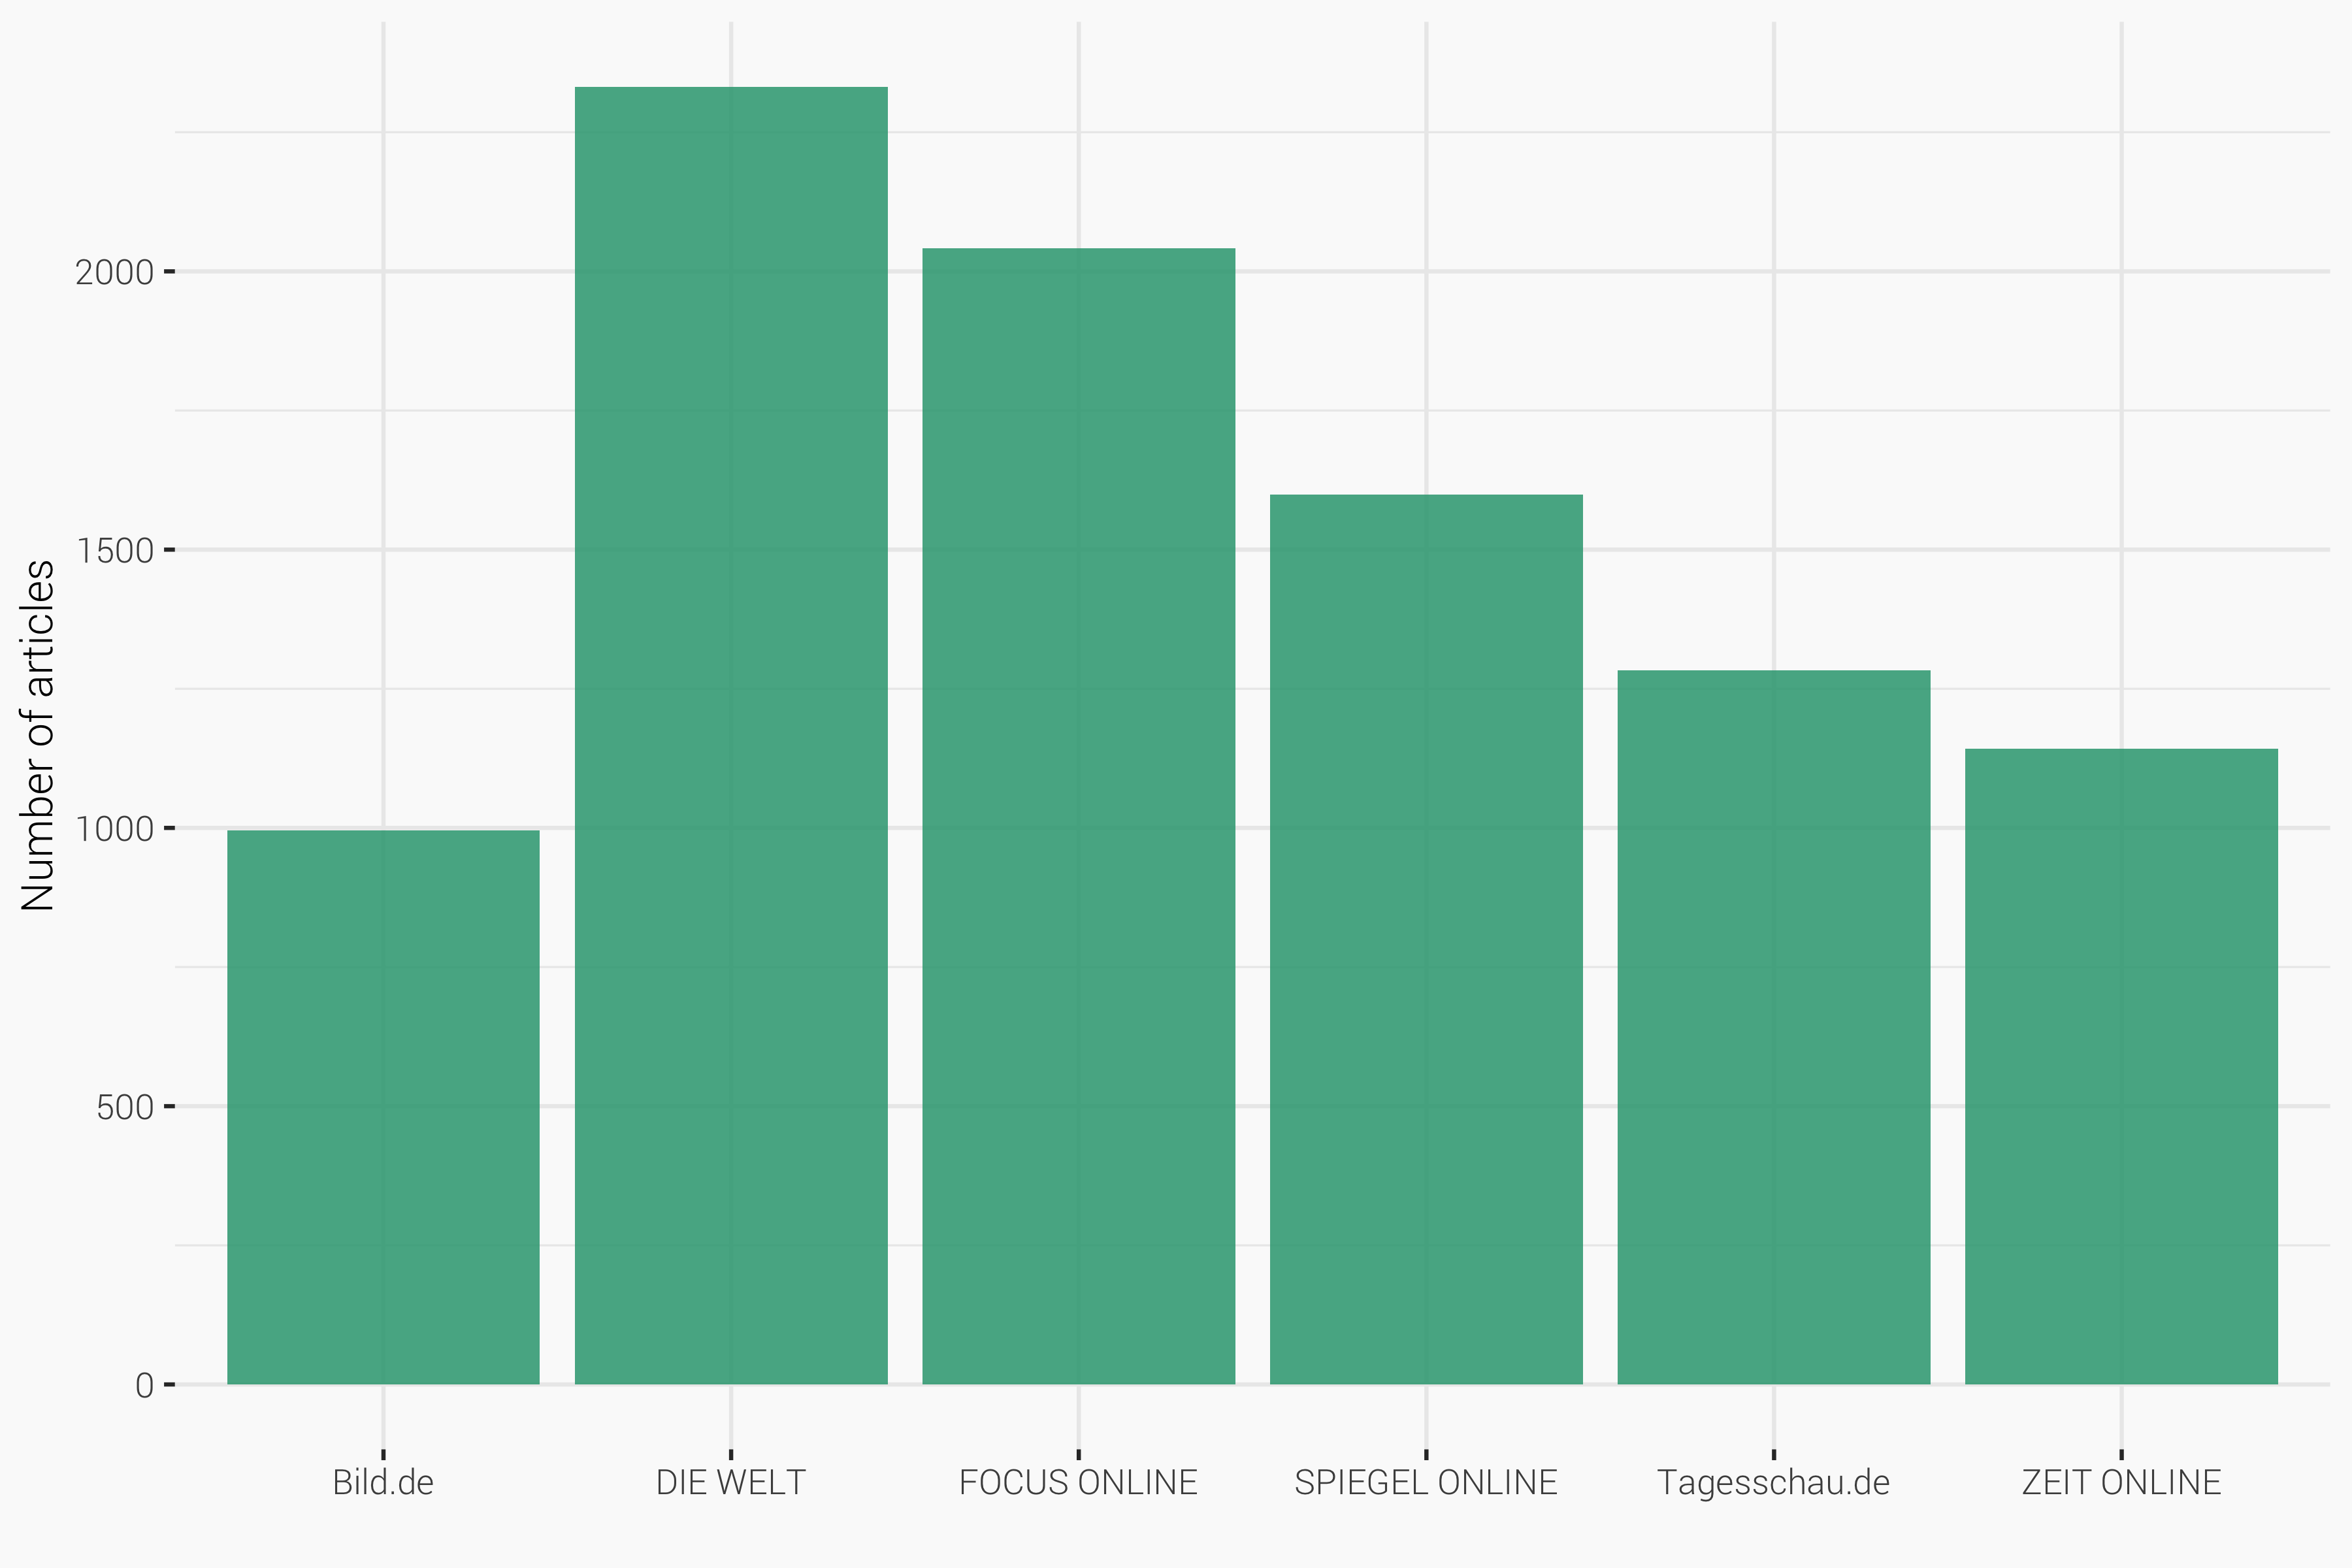
\includegraphics[width=\textwidth]{../figs/bar.png}
			\caption{... by news source}
			\label{fig_distr2}
		\end{subfigure}
	\end{center}
\end{figure}

Looking at the histograms of the word counts (Figure \ref{fig_wordcount}), it becomes evident that most of the articles have a word length between 200 and 1000 words (articles with less than 200 words were filtered out in advance, as these are mostly reader comments). The distribution at Bild.de, DIE WELT, FOCUS ONLINE and stern.de is left-skewed, whereby stern.de has comparatively many articles with a word length of over 2000. 

\begin{figure}[H]
	\caption{Word Count}
	\begin{center}
		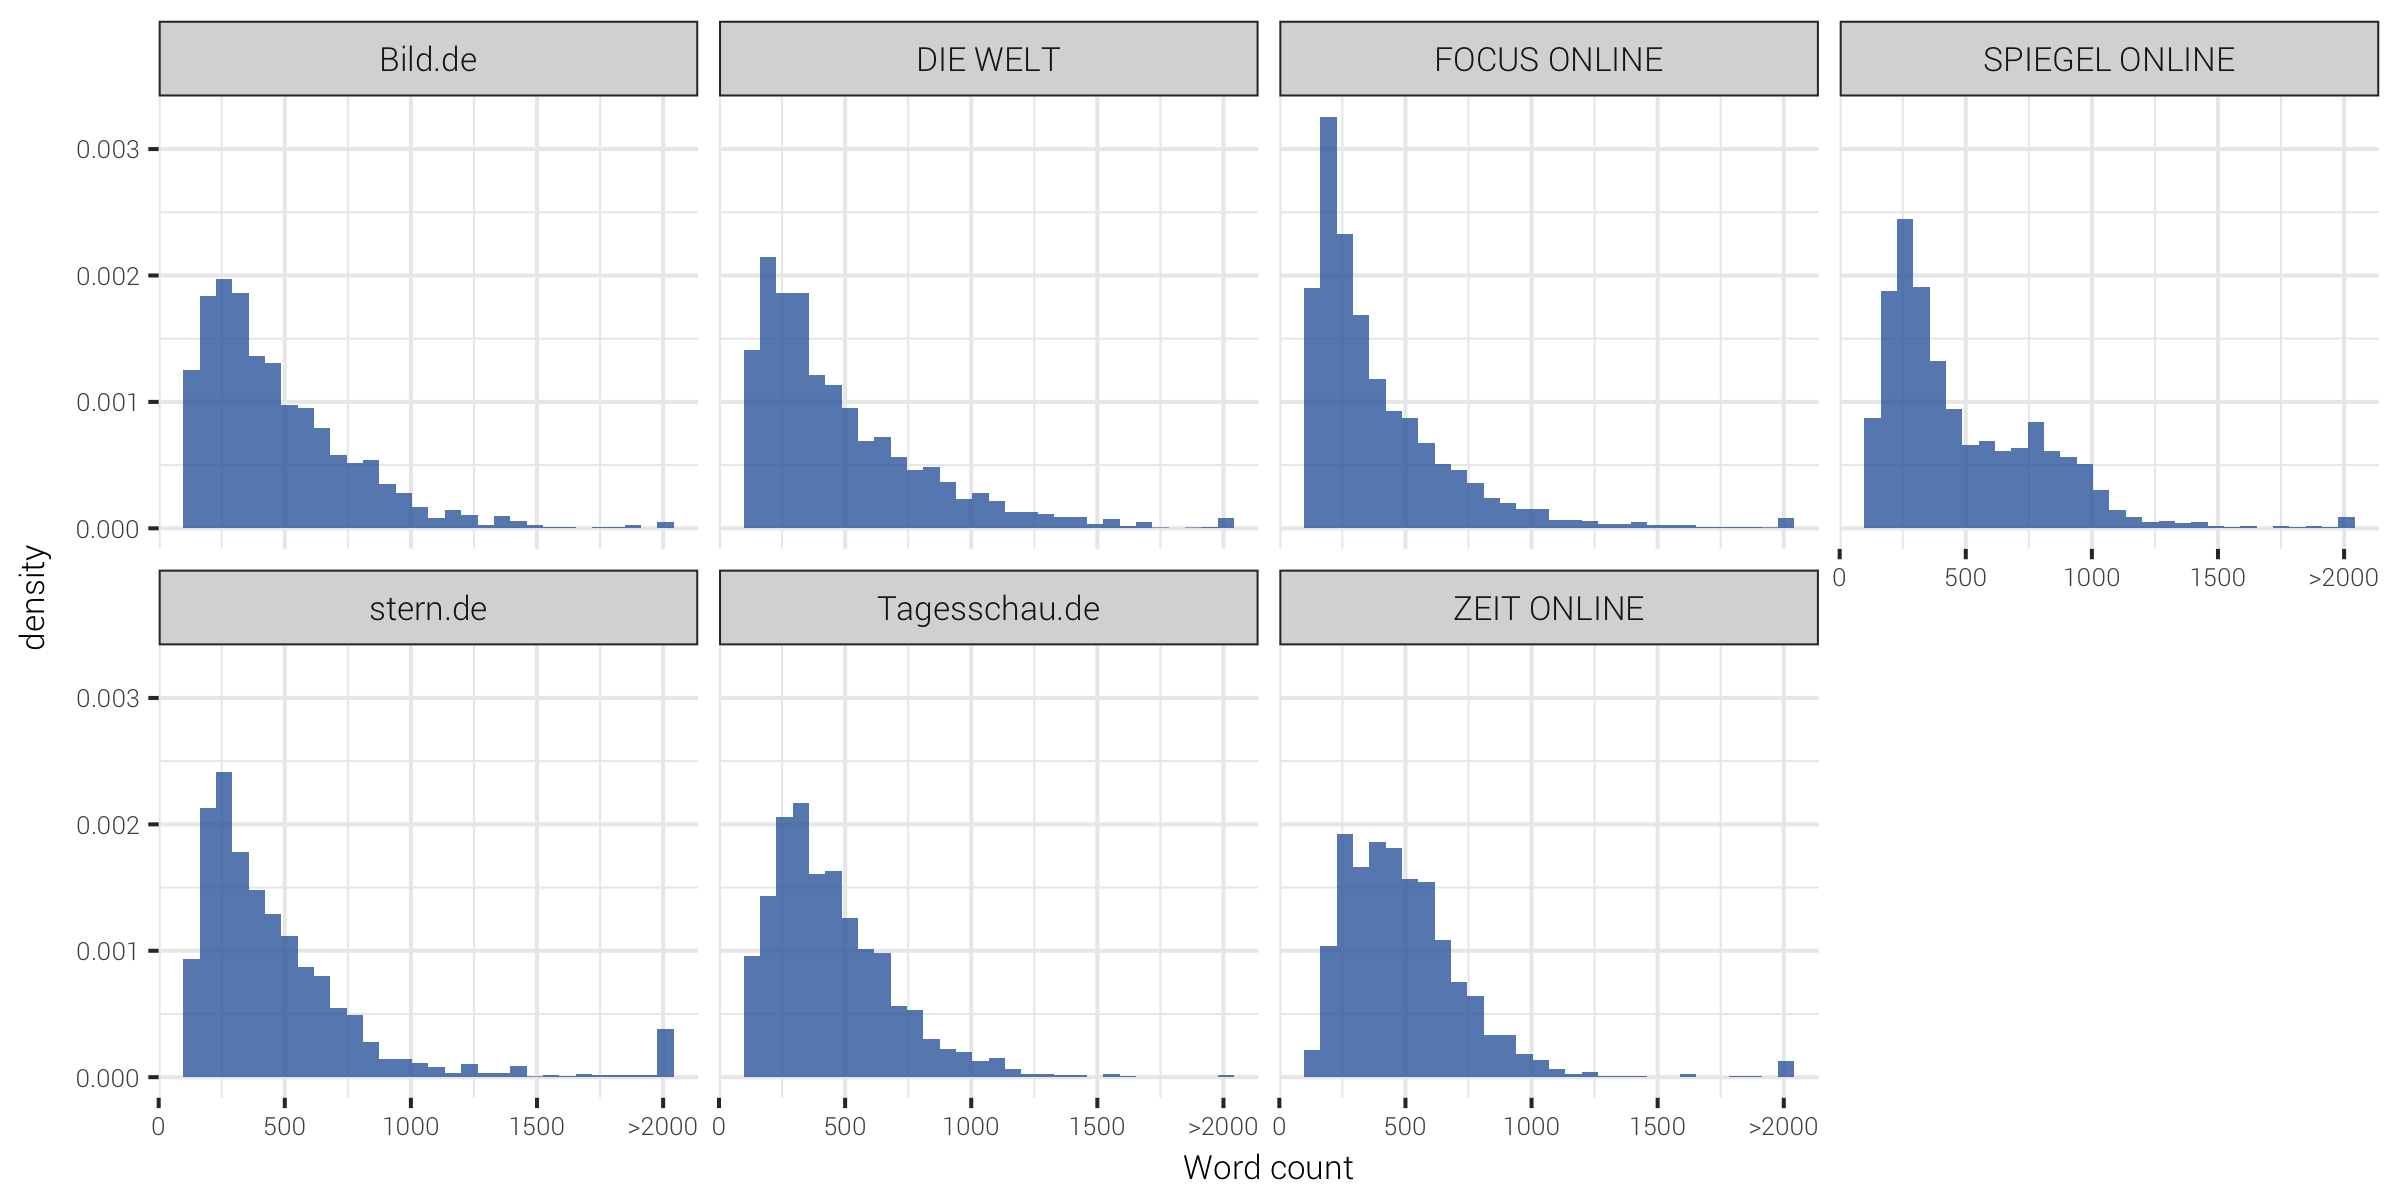
\includegraphics[width=\textwidth]{../figs/wordcount.png}
		\label{fig_wordcount}
	\end{center}
\end{figure}

The longest article at Tagesschau.de has 2006 words, nevertheless the median value is comparatively large (see Table \label{t_wordcount}). ZEIT ONLINE has the highest median value of 459 words. 

% latex table generated in R 3.4.2 by xtable 1.8-2 package
% Wed May  9 00:33:54 2018
\begin{table}[ht]
\centering
\begin{tabular}{rlrrrrrrr}
  \hline
 & group1 & n & mean & sd & median & min & max & se \\ 
  \hline
1 & Bild.de & 1277.00 & 475.20 & 319.22 & 394.00 & 121.00 & 3710.00 & 8.93 \\ 
  2 & DIE WELT & 3179.00 & 507.88 & 614.28 & 377.00 & 121.00 & 14507.00 & 10.89 \\ 
  3 & FOCUS ONLINE & 2660.00 & 402.68 & 330.86 & 299.00 & 121.00 & 5647.00 & 6.42 \\ 
  4 & SPIEGEL ONLINE & 1817.00 & 498.96 & 333.23 & 387.00 & 121.00 & 3304.00 & 7.82 \\ 
  5 & stern.de & 2922.00 & 518.09 & 622.99 & 376.50 & 121.00 & 9287.00 & 11.53 \\ 
  6 & Tagesschau.de & 1644.00 & 450.34 & 242.93 & 397.50 & 121.00 & 2006.00 & 5.99 \\ 
  7 & ZEIT ONLINE & 1437.00 & 510.98 & 377.85 & 459.00 & 121.00 & 8015.00 & 9.97 \\ 
   \hline
\end{tabular}
\caption{Summary statistics of text length} 
\end{table}


To summarize the content of the texts, wordclouds help to get a first impression, as the frequency of words in a corpus are represented by their size. Intuitively the term frequency (tf) of a word is a measure of how important that word may be. The word cloud in Figure \ref{fig_wordcloud1} is derived from all articles within the dataset. As can be seen, problems arise with words that are highly frequent. For example "die" ("the"), "und" ("and"), and "in" ("in") are extremely common but unrelated to the quantity of interest. These terms, often called stop words, are important to the grammatical structure of a text, but typically don't add any additional meaning and can therefore be neglected. A common strategy to reduce the number of language elements is to pre-process the text by imposing some preliminary restrictions (stop-word removal and stemming) based on the nature of the data (twitter text, newspaper articles, speeches, etc.) \citep{gentzkow_text_2017}. In fact, to use text as data and reduce the dimensionality to avoid unnecessary computational complexity and overfitting, pre-processsing the text is a central task in text mining \citep{bholat_text_2015}.  

\begin{figure}[H]
	\caption{Word Cloud (whole corpus)}
	\begin{center}
		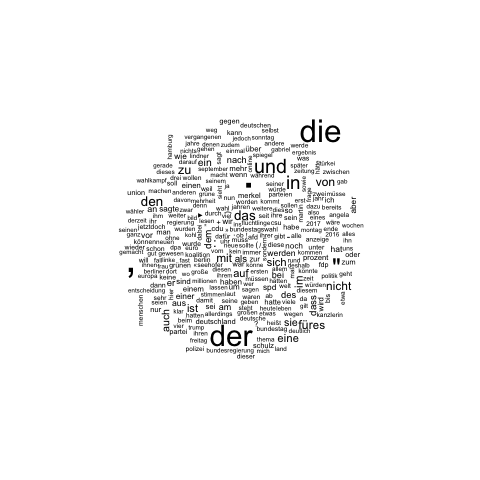
\includegraphics[width=0.8\textwidth]{../figs/wordcloud.png}
		\label{fig_wordcloud1}
	\end{center}
\end{figure}

Stemming is a process by which different morphological variants of a word are traced back to their common root. For example, "voting" and "vote" would be treated as two instances of the same token after the stemming process. There are many different techniques for the stemming process. I apply the widely used Porter-Stemmer algorithm, which is based on a set of shortening rules that are applied to a word until it has a minimum number of syllables.\footnote{https://tartarus.org/martin/PorterStemmer/} To remove distorting words, the pre-defined stop word list from the Snowball project\footnote{http://snowball.tartarus.org/algorithms/german/stop.txt} together with a customized list of stop-words is used. Additionally punctuation character (e.g. ., ,, !, ?, etc.) and all numbers are removed from our corpus. After completing this steps we were left with 68.576 unique terms in our vocabulary. The following wordclouds are derived from the corpus for each news provider. It becomes evident that these are texts discussing domestic policy issues. The SPD in particular seems to be highly frequent. However, at first glance, there are no obvious differences between the corpus of the different news provider.  

% --------------------
% Document-term-matrix
% --------------------
To use the data for statistical analysis, the next step is to divide the whole corpus into individual documents and to represent these documents as a finite list of unique terms. In this setting, each news article represents a document $d$, whereby each of these documents can be assigned to a news website. Next, for each document $d \in \lbrace 1,...,D \rbrace$ the number of occurrences of term $v$ in document $d$ is computed, to obtain the count $x_{d,v}$, where each unique term in the corpus is indexed by some $v \in \lbrace 1,...,V \rbrace$ and where $V$ is the number of unique terms. The $D$ x $V$ matrix $\boldsymbol{X}$ of all such counts is called the document-term matrix. This representation is often referred to as the bag of words model, since the order in which words are used within a document is disregarded. The sum of all documents forms what is called the corpus.

\begin{figure}[H]
	\caption{Word Clouds}
	\begin{center}
		\begin{subfigure}[normla]{0.3\textwidth}
			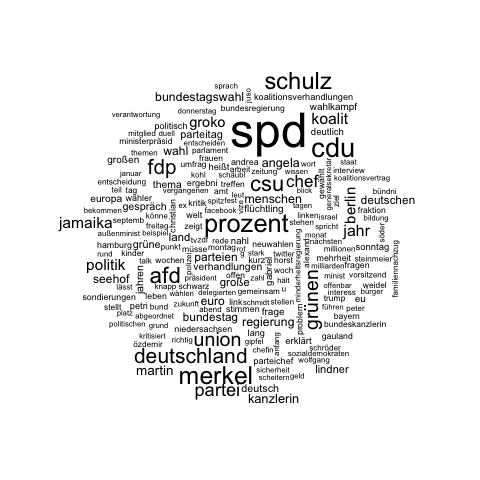
\includegraphics[width=\textwidth]{../figs/wordcloud_Bild.png}
			\caption{Bild.de}
		\end{subfigure}
		\begin{subfigure}[normla]{0.3\textwidth}
			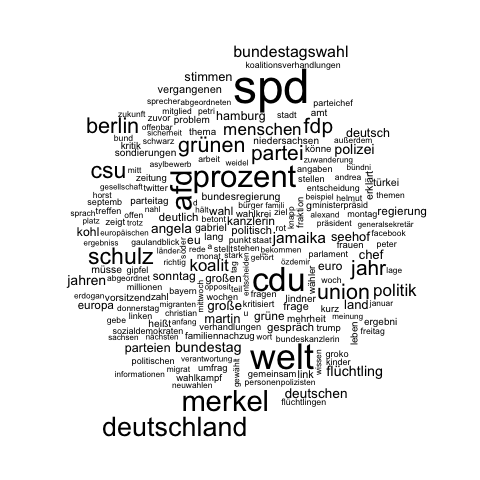
\includegraphics[width=\textwidth]{../figs/wordcloud_DIEWELT.png}
			\caption{DIE WELT}
		\end{subfigure}
		\begin{subfigure}[normla]{0.3\textwidth}
			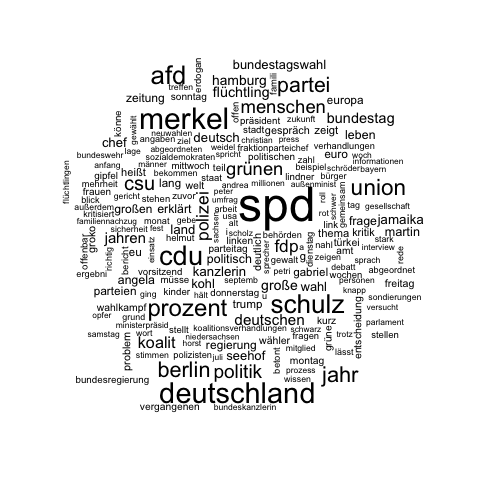
\includegraphics[width=\textwidth]{../figs/wordcloud_FOCUSONLINE.png}
			\caption{FOCUS ONLINE}
		\end{subfigure}
		\begin{subfigure}[normla]{0.3\textwidth}
			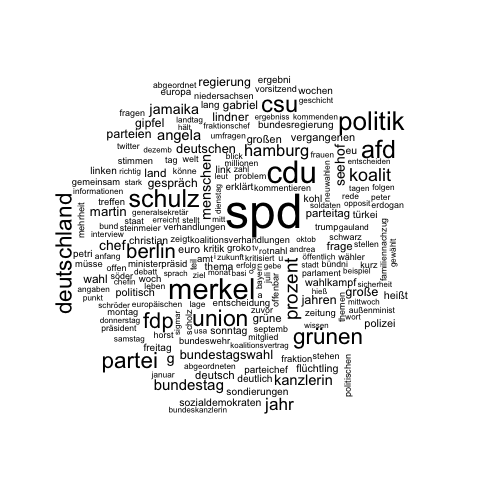
\includegraphics[width=\textwidth]{../figs/wordcloud_SPIEGELONLINE.png}
			\caption{SPIEGEL ONLINE}
		\end{subfigure}
		\begin{subfigure}[normla]{0.3\textwidth}
			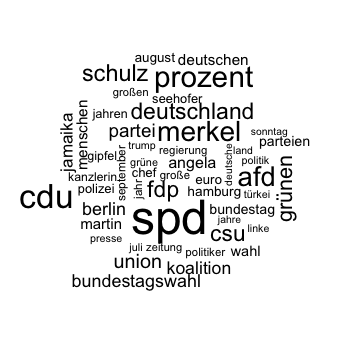
\includegraphics[width=\textwidth]{../figs/wordcloud_stern.png}
			\caption{Stern.de}
		\end{subfigure}
		\begin{subfigure}[normla]{0.3\textwidth}
			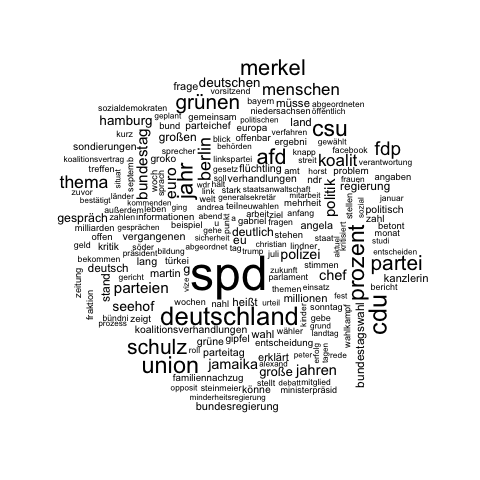
\includegraphics[width=\textwidth]{../figs/wordcloud_Tagesschau.png}
			\caption{Tagesschau.de}
		\end{subfigure}
		\begin{subfigure}[normla]{0.3\textwidth}
			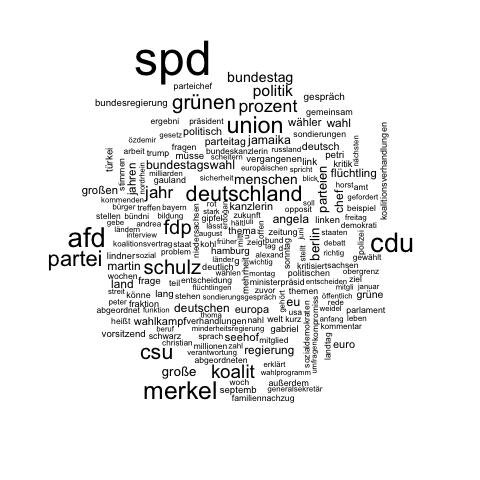
\includegraphics[width=\textwidth]{../figs/wordcloud_ZEITONLINE.png}
			\caption{ZEIT ONLINE}
		\end{subfigure}
	\end{center}
\end{figure}
 
% ----------------------
% Structural topic Model
% ----------------------
\section{The structural topic model}\label{ch_model}

To find out the latent structure of each document, a structural topic model (STM) is estimated. In general, topic models formalize the idea that documents are formed by hidden variables (topics) that generate correlations among observed terms. They belong to the group of unsupervised generative models, meaning that the true attributes (topics) cannot be observed. One crucial assumption to be made for such models is the number of topics that occur over the entire corpus ($K$). 

Each individual topic potentially contains all of the unique terms within the vocabulary $V$ with different probability. Therefore, each topic $k$ can be represented as a probability vector $\phi_k$ over all unique terms $V$. Simultaneously, each individual document $d$ in the corpus can be represented as a probability distribution $\theta_d$ over the $K$ topics. To generate each individual word $w_{d,n}$ in a document $d$ for the $n^{th}$ word-position, a topic allocation $z_{d,n}$ is drawn from the topic distribution for that document $\theta_d$. Then, a word is drawn from the term distribution for the selected topic $\phi_{z_{d,n}}$.\footnote{A more detailed description of the generative process of the STM can be found in Section \ref{ch_generativeProcess}}

The STM developed by \citet{roberts_model_2016} is a recent extension of the standard topic modeling technique, labeled as latent Dirichlet allocation (LDA), which refers to the Bayesian model in \citet{blei_latent_2003} that treats each word in a topic and each topic in a document as generated from a Dirichlet - distributed prior.\footnote{See also \citet{griffiths_probabilistic_2002}, \citet{griffiths_finding_2004} and \citet{hofmann_probabilistic_1999}. \citet{pritchard_inference_2000} introduced the same model in genetics for factorizing gene expression as a function of latent populations.} Since its introduction into text analysis, LDA has become hugely popular and especially useful in political science.\footnote{see \citet{blei_probabilistic_2012}, \citet{grimmer_text_2013} and \citet{wiedmann_text_2016} for an overview in social science and \citet{gentzkow_text_2017} give an overview of text mining applications in economics.} \citet{wiedmann_text_2016} uses topic model methods on large amounts of news articles from two german newspapers published between 1959 and 2011, to reveal how democratic demarcation was performed in Germany over the past six decades. \citet{paul_cross-collection_2017} compares editorial differences between media sources, using cross-collection latent Dirichlet allocation (ccLDA), an LDA-based approach that incorporates differences in document metadata. They use a dataset of 623 news articles from August 2008 from two American media outlets - msnbc.com and foxnews.com - to compare how they discuss topics. Reviewing the top words of the word-topic distribution, they find some content differences between the two media sources under review. 

The STM allows to incorporate document specific covariates (e.g. the author or date of a document). The model has been applied to multiple academic fields: \citet{roberts_structural_2014} uses STM to analyze open-ended responses from surveys and experiments, \citet{farrell_corporate_2016} applies the model to scientific texts on climate change, revealing links between corporate funding and the framing of scientific studies. \citet{mishler_using_2015} show that "STM can be used to detect significant events such as the downing of Malaysia Air Flight 17" when applied to twitter data. Another study shows how STM can be used to explore the main international development topics of countries’ annual statements in the UN General Debate and examine the country-specific drivers of international development rhetoric \citep{baturo_what_2017}. \citet{mueller_reading_2016} use newspaper text to predict armed conflicts in different regions. They use the estimated topic shares in linear fixed effects regression to forecast conflict out-of-sample. \citet{roberts_navigating_2016} use STM to examine the role of partisanship in topical coverage using a corpus of 13,246 posts that were written for 6 political blogs during the course of the 2008 U.S. presidential election. With the aim of revealing the effect of partisan membership on topic prevalence, each blog is assigned to be either liberal or conservative. To explore the differences between the two, they look at the expected proportion of topic and examine the posts most associated with a respective topic. This approach is similar to \citet{roberts_model_2016}. 

% Topic Modeling
% --------------
\subsection{Generative Process of STM}\label{ch_generativeProcess}

 As mentioned above, the STM allows to incorporate observed document metadata which is able to affect both topical prevalence and topical content. These assumptions are reflected in the prior distributions. The following describes the generative process for filling the $n^{th}$ word-position in document $d$ in the case of the STM \citep{roberts_structural_2013}: As in the case of conventional models, first a specific topic $z_{dn}$ is assigned, according to the topic distribution for that document $\theta$ through the process:

\begin{equation}
	z_{dn}|\theta_d \sim \textrm{Multinomial}(\theta_d).
\end{equation}

To incorporate the covariate values for that document, a topic-prevalence vector $\theta_d$ is drawn from a logistic-normal distribution:

\begin{equation}
	\theta_d|y_{d\gamma},\Sigma \sim \textrm{LogisticNormal}(\mu = y_{d\gamma}\Sigma),
\end{equation}

where $y_d\gamma$ lists the values of all metadata covariates for document $d$, where $\gamma$ relates these covariate values to the topic-prevalence. The structure of $\Sigma$ implies the possibility of correlations across documents in the topic-prevalence vector. 

Conditional in the topic chosen ($z_{dn}$), a specific word $w_{dn}$, is chosen from the overall corpus vocabulary $V$, using the following process:

\begin{equation}
	w_{dn}|z_{dn},\phi_{dkv} \sim \textrm{Multinomial}(\phi_{dk1},...,\phi_{dkV}),
\end{equation}

where the word probability $\phi_{dkv}$ is parameterized in terms of log-transformed rate deviations from the rates of a corpus-wide background distribution $m_v$ \citep{roberts_structural_2013}. The log-transformed rate deviations can then be specified by a collection of parameters $\lbrace \boldsymbol{\kappa} \rbrace$, where $\kappa^{(t)}$ is a $K$-by-$V$ matrix containing the log-transformed rate deviations for each topic $k$ and term $v$, over the baseline log-transformed rate for term $v$. This matrix is the same for all $A$ levels of covariates. To put it differently, $\kappa^{(t)}$ indicates the importance of the term $v$ given topic $k$ regardless of the covariates. Similarly, $\kappa^{(c)}$ is a $A$-by-$V$ matrix, indicating the importance of the term $v$ given the covariate level $c$ regardless of the topic. Finally, $\kappa^{(i)}$ is a $A$-by-$K$-by-$V$ matrix, collecting the covariate-topic effects:

\begin{equation}
	\phi_{dkv}|z_{dn}=\frac{\textrm{exp}(m_v+\kappa^{(t)}_{kv},\kappa^{(c)}_{y_dv}+\kappa^{(i)}_{y_dkv})}{\sum_v \textrm{exp}(m_v+\kappa^{(t)}_{kv},\kappa^{(c)}_{y_dv}+\kappa^{(i)}_{y_dkv})}.
\end{equation}

The STM maximizes the posterior likelihood that the observed data were generated by the above data-generating process using an iterative approximation-based variational expectation-maximization algorithm\footnote{A technical description of this maximization process can be found in \citet{roberts_model_2016}} available in R's stm package \citep{roberts_stm:_2016}. 

This process generates two posterior distribution parameter: 

\begin{enumerate}
	\item $\phi$ is a $K$-by-$V$ matrix (where $K=$ number of topics and $V=$ vocabulary), where the entry $\phi_{kvc}$ can be interpreted as the probability of observing the $v$-th word in topic $k$ for the covariate level $c$ (the news website). 
	\item $\theta$ is a $D$-by-$V$ matrix (where $D=$ number of documents and $V=$ vocabulary) of the document-topic distributions, where the entry $\theta_{dk}$ can be interpreted as the proportion of words in document $d$ which arise from topic $k$, or rather as the probability that document $d$ deals about topic $k$. 
\end{enumerate}

In Section \ref{subsection_topic} $\theta$ is used to estimate the conditional expectation of topic prevalence for given document characteristics. In order to calculate the sentiment value in Section \ref{subsection_tone} each document $d$ is assigned to the topic with the highest probability ($\max (\theta_{k})$ for each document $d$).

% ----------------------
% Model Selection
% ----------------------
\subsection{Model and parameter selection}

Inference of mixed-membership models, such as the one applied in this paper, has been a thread of research in applied statistics in the past few years \citep{blei_latent_2003} \citep{erosheva_mixed-membership_2004} \citep{braun_variational_2010}. Topic models are usually imprecise as the function to be optimized has multiple modes, such that the model results can be sensitive to the starting values (e.g. the number of topics). Since an ex ante valuation of a model is hardly possible, I compute a variety of different models and compare their posterior probability. This enables me to check how results vary for different model solution \citep{roberts_navigating_2016}. I then cross-checked some subset of assigned topic distributions to evaluate whether the estimates align with the concept of interest \citep{gentzkow_text_2017}. These manual audits are applied together with numeric optimization based on the topic coherence measure suggested by \citet{mimno_optimizing_2011}. 

This process revealed that a model with 50 topics best reflects the structure in the corpus. Furthermore, the news website of the article is used as covariates in the topic prevalence and the topical content. In other words, the corresponding news website of an article influences the probability distribution of topics and how the topics are discussed. 

% ----------------------
% Model Results
% ----------------------
\section{Empirical Evaluation}\label{ch_empirical}

This section summarizes the results of the STM. Subsequently "the two T's" (Topic and Tone) of the corpus are analyzed according to the following approaches: (1) The document-topic probability $\theta_{dk}$ is used, to estimate the conditional expectation of topic prevalence for given document characteristics (See section \ref{subsection_topic}). A set of topics is selected, that most distinctly discuss a particular party or a topic related to the federal elections. (2) Articles that are assigned to the selected topics with the highest probability are then used to conduct a dictionary-based analysis (see section \ref{subsection_tone}). In order to check whether the sentiment value of certain topics are correlated with the results of voting preferences, the cross correlation function between these two concepts is calculated in \ref{ch_correlation}.

\subsection{Topic}\label{subsection_topic}

In order to get an initial overview of the results, Figure \ref{fig_topic_proportion} displays the topics ordered by their expected frequency across the corpus. To assign a label to each topic, I looked at the most frequent words in that topic and the most representative articles \citep{roberts_model_2016}. 

It becomes apparent that topic 4 about the coalition talks between CDU/CSU and SPD - the "Grand coalition" or "GroKo" - is the topic with the highest expected frequency in the whole corpus, followed by the topic about the so-called Jamaica parties (CDU/CSU, FDP and B90/Die Grünen), which was the first alternative to be negotiated directly after the elections.  

\begin{figure}[H]
	\begin{center}
	\caption{Expected topic proportion}
		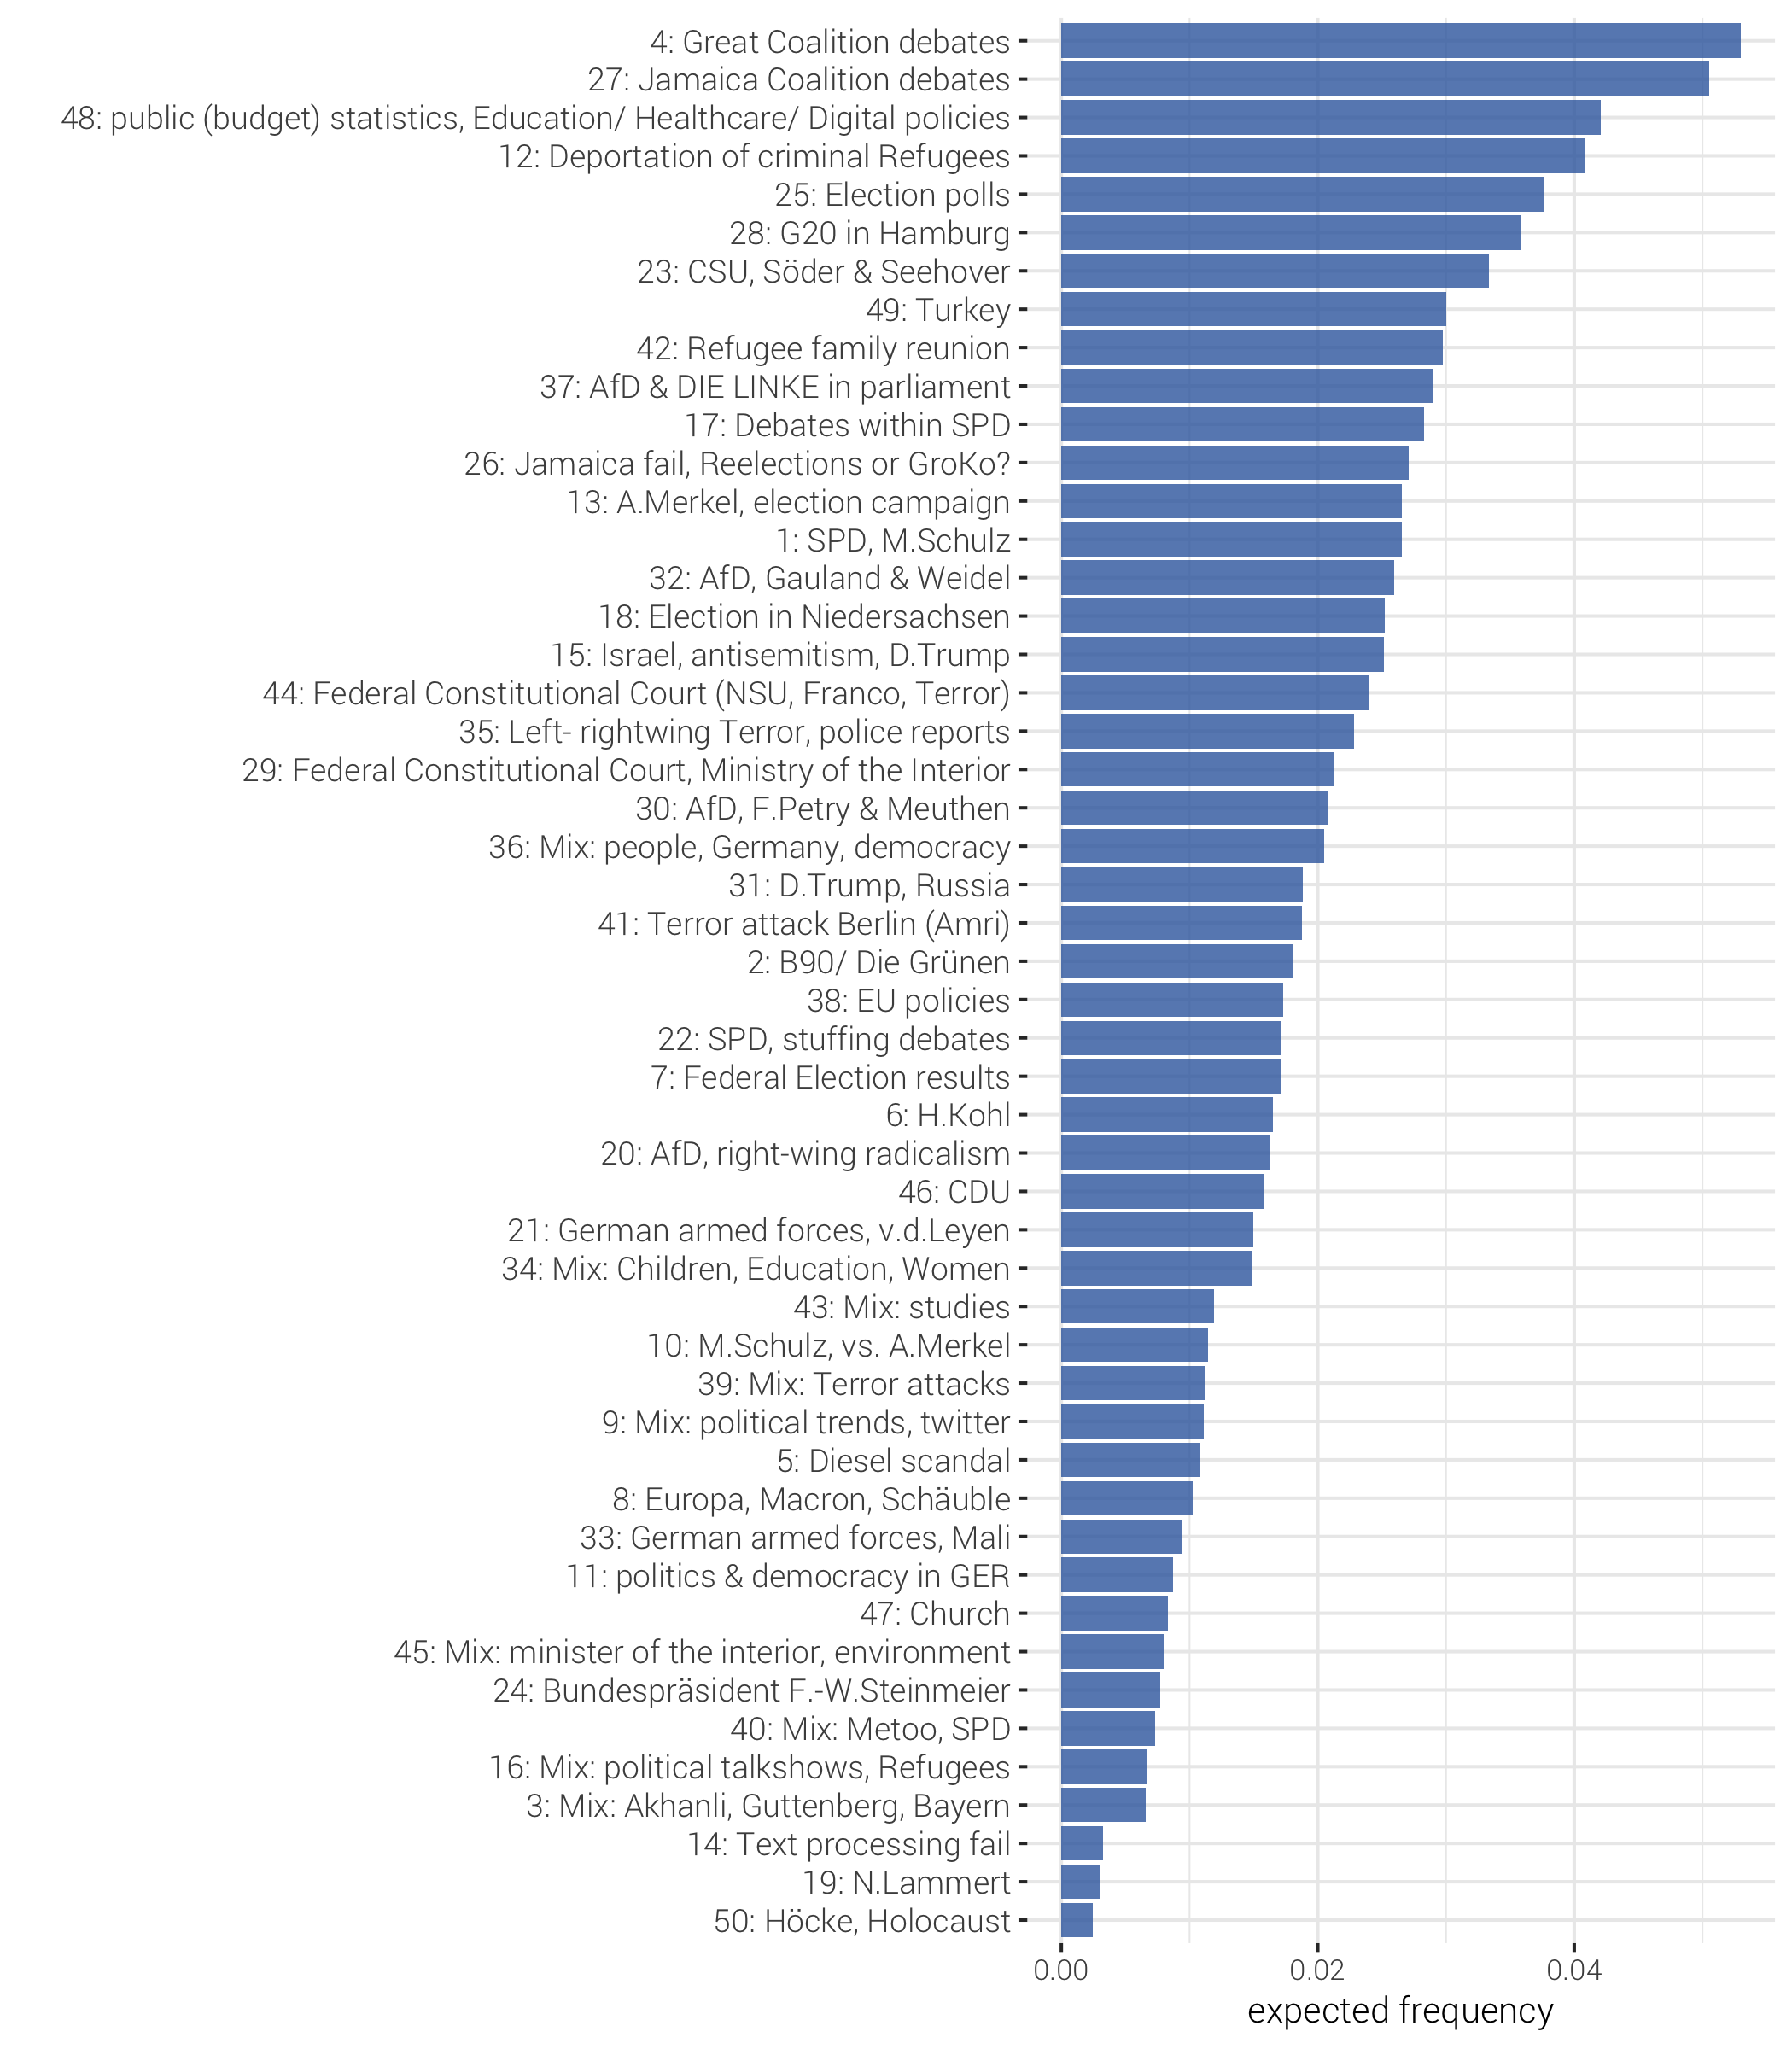
\includegraphics[width=\textwidth,keepaspectratio]{../figs/topic_proportion.png}
		\label{fig_topic_proportion}
\end{center}
\end{figure}

The remaining analysis is limited to topics closely related to one or more parties. For this reason, the following topics were selected. The most frequent words of these topics at each news website can be seen in Appendix \ref{apx_tf}: 

\begin{enumerate}
	\item Topic 1: About the SPD, mainly about the election campaign and Martin Schulz as candidate for the chancellor.	
	\item Topic 2: About B90/Die Grünen, mainly covering issues regarding the party's personell debates.
	\item Topic 4: Covering the debates about the great coalition talks, mainly after the failure of the Jamaica coalition talks.
	\item Topic 13: About Angela Merkel, mainly right before the election. 
	\item Topic 17: Covering votes within the SPD, mainly regarding the vote about a possible coalition with CDU/CSU/CSU ("GroKo").	
	\item Topic 20: About the AfD, mainly about their relation to right-wing extremist groups.
	\item Topic 22: About SPD, mainly covering issues regarding the party's personell debates
	\item Topic 23: About issues regarding the CSU, mainly about the competition between Horst Seehofer and Markus Söder and the negotiations with the CDU/CSU.
	\item Topic 26: Discussing the failure of the Jamaica coalition talks and the two possible alternatives: Reelections or a great coalition.
	\item Topic 27: Covering the Jamaica coalition talks, mainly focusing on the smaller players Bündnis B90/Die Grünen and FDP.	
	\item Topic 30: About the AfD, mainly about the resignation of Frauke Petry and Jörg Meuthen.
	\item Topic 32: About the AfD, mainly about Alice Weidel and Alexander Gauland, voted as parliamentary party leaders after the resignation of Frauke Petry.
	\item Topic 37: Covering debates of AfD and DIE LINKE in the parliament (Deutscher Bundestag).
	\item Topic 46: Covering issues regarding the CDU/CSU.
\end{enumerate}   

To estimate the differences of topic prevalence of the mentioned topics for the different websites, a linear model is calculated for each topic $k$, where the documents are observations, the dependent variable is the posterior probability of the respective topic ($\theta_{d}$) and the covariates are dummy variables that are 1 if the document was published by the respective website and 0 otherwise (see equation \ref{eq_1}). As the dependent variable is a vector containing proportions that sum up to 1, the QR decomposition of the model is computed prior to the estimation of the coefficients. To incorporate uncertainty in the dependent variable, a set of topic proportions are drawn from the variational posterior (the unnormalized topic proportions) repeated times. Then, the coefficients are computed as the average over all results \citep{roberts_model_2016}.

\begin{equation}\label{eq_1}
\begin{split}
	\theta_{d}=\beta_0+\beta_1 x_{\text{FOCUS ONLINE,d}}+\beta_2 x_{\text{SPIEGEL ONLINE,d}}+\\
	\beta_3 x_{\text{stern.de,d}}+\beta_4 x_{\text{Tagesschau.de,d}}+\beta_5 x_{\text{DIE WELT,d}}+\\
	\beta_6 x_{\text{ZEIT ONLINE,d}}+\epsilon
\end{split}
\end{equation}

Figure \ref{fig_estimateEffects} shows the regression results for the above selected topics (See Appendix \ref{apx_coeff} for the result tables). The coefficients indicate the deviation from the base value of Bild.de. Starting from above it becomes apparent that the topic prevalence of topic 46 (regarding the CDU/CSU) is significantly less for Tagesschau.de and Stern.de. The other media do not show any significant difference to Bild.de for this topic. The opposite is true for topic 37: With the exception of Stern.de and DIE WELT, topic prevalence for this topic is significantly higher for all media than for Bild.de. With the following two topics on AfD it is striking that the topic prevalence at Tagesschau.de is significantly lower compared to Bild.de. The topics concerning the Jamaican coalition (topic 27) and the failure (topic 26) seem to be discussed most likely at Bild.de. The case is different for the CSU issue (Topic 23), where SPIEGEL ONLINE has the highest probability. The same applies to the topic related to the personnel debates of the SPD (22). However, Bild.de has the highest topic prevalence for the topic related to votes within the SPD, especially the vote on the grand coalition. The same applies to the topic regarding the SPD in general and Martin Schulz in particular (1). Overall, topics concerning the SPD seem to be more frequent at Bild.de than in the other media. Moreover, the distribution of topics at FOCUS ONLINE seems to be the most similar to that of Bild.de, while the biggest differences exist between Bild.de and Tagesschau.de. 

\begin{figure}[H]
	\caption{Regression results}
		\begin{center}
			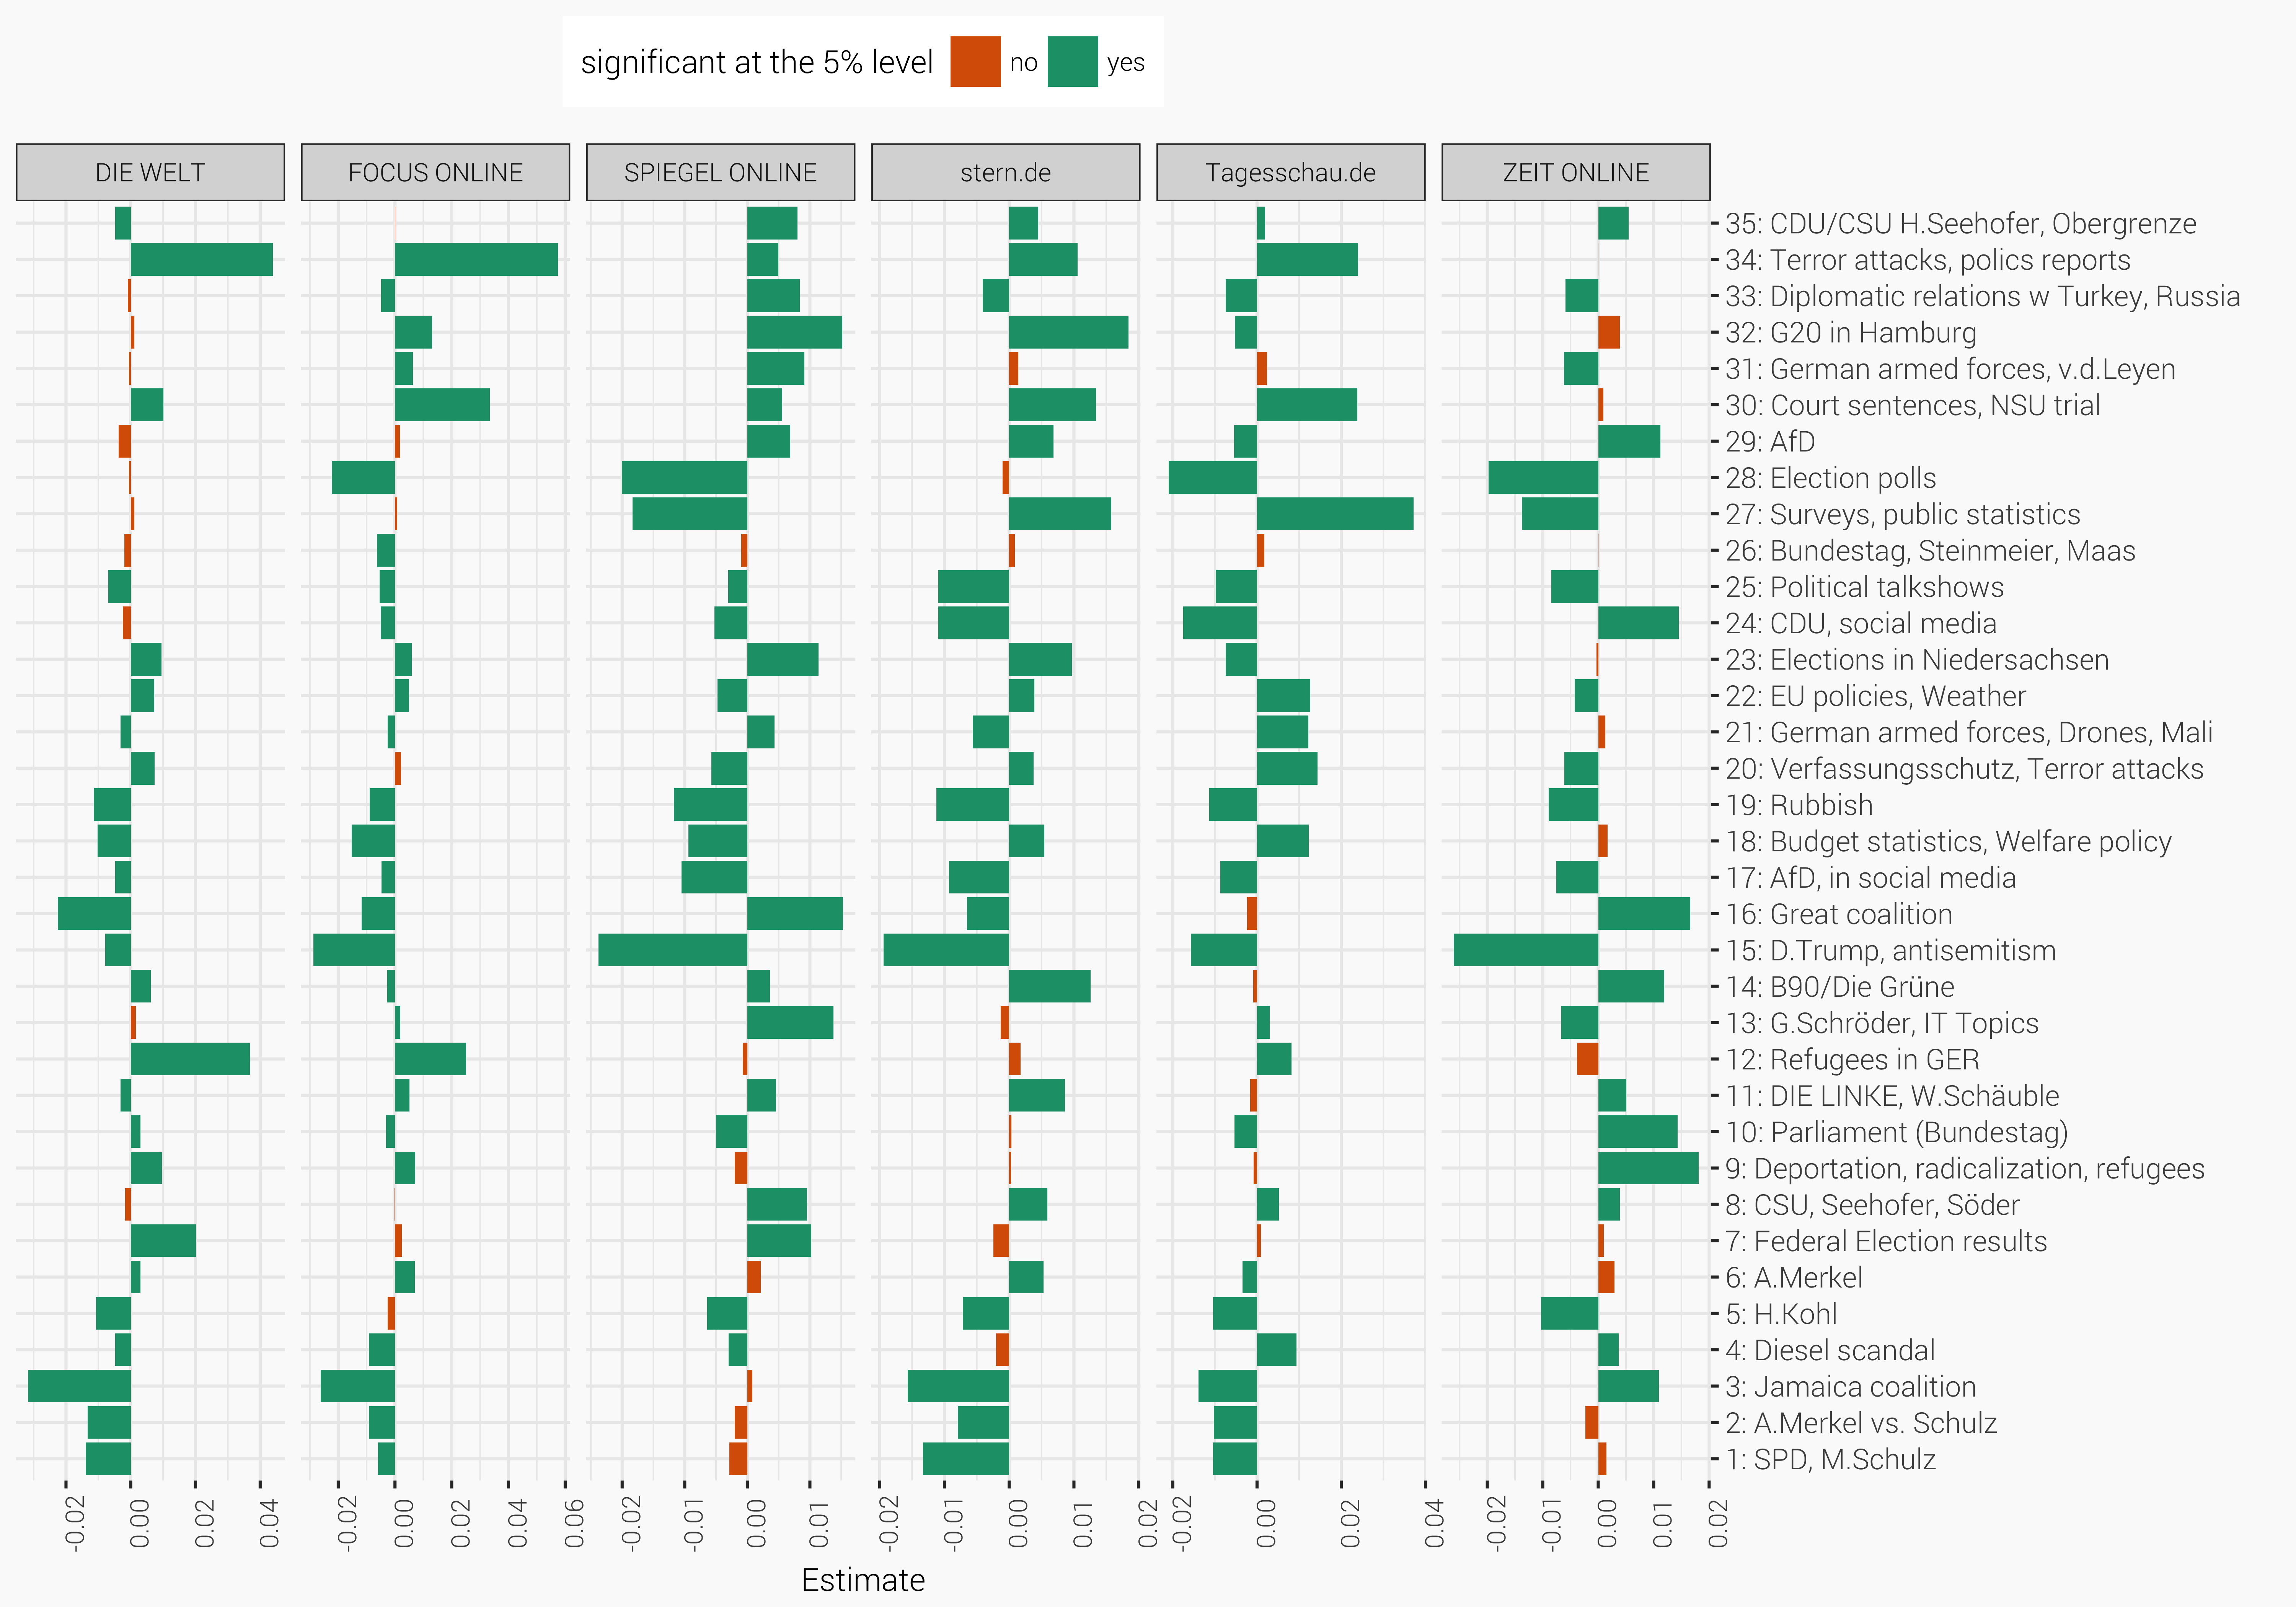
\includegraphics[width=\textwidth,keepaspectratio]{../figs/estimates.png}
		\end{center}
	\label{fig_estimateEffects}
\end{figure}

\subsection{Tone}\label{subsection_tone}

The sentiment analysis is performed with the documents for which one of the above topics has the highest posterior probability and if this probability is greater than 30\%. A dictionary-based method is then applied on the remaining 5611 documents with the aim to measure the tone (or sentiment) of a document. The idea of a sentiment analysis is to determine the attitude of a writer toward the overall tonality of a document. To conduct such an analysis, a lists of words (dictionary) associated with a given emotion, such as negativity is pre-defined by the analyst. The document is then deconstructed into individual words and the frequencies of words contained in a given dictionary are calculated. 

Such lexical or “bag-of-words” approaches are widely presented in the finance literature to determine the effect of central banks' monetary policy communications on asset prices and real variables (\citet{nyman_news_2018} \citep{tetlock_giving_2007}, \citep{tetlock_more_2008}). \citet{hansen_shocking_2016} use a similar approach to measure "the two Ts" (Topic and tone). They explore the effects of FOMC (Federal Open Market Committee) statements on both market and real economic variables. To understand the multi-dimensional information a statement is transmitting, they apply LDA on a corpus of 142 FOMC decision statements split into sentences (topic). They then measure how the central bank is talking about that topic, using a dictionary approach (tone). To calculate their score, they subtract the negative words from the positive words und divide this by the number of total words of the statement. A similar score is used by \citet{nyman_news_2018}, who measure the effect of narratives and sentiment of financial market text-based data on developments in the financial system. They count the number of occurrences of excitement words and anxiety words and then scale these numbers by the total text size as measured by the number of characters.

The present paper uses a dictionary that lists words associated with positive and negative polarity weighted within the interval of $[-1; 1]$. SentimentWortschatz\footnote{SentiWS for short. available here: http://wortschatz.uni-leipzig.de/de/download}, is a publicly available German-language resource for sentiment analysis, opinion mining etc. The current version of SentiWS (v1.8b) contains 1,650 positive and 1,818 negative words, which sum up to 15,649 positive and 15,632 negative word forms including their inflections, respectively. The sentiment score for each document $d$ is calculated  based on the weighted polarity values for a word, defined on an interval between -1 and 1. The score is then calculated from the sum of the words in a document (which can be assigned to a word from the dictionary) divided by the total number of words in that document:
 
\begin{equation}
	\text{SentScore}_d = \frac{|\text{positive polarity score}_d| - |\text{negative polarity score}_d|}{|\text{TotalWords}_d|}
\end{equation}

Figure \ref{fig_sentscore_monthly} shows the results of the analysis for each topic on a monthly basis, aggregated on all newspapers. Each sentiment value is weighted by the relative share of the topic in the overall reporting of that month.

Some conclusions can be drawn from this illustration. First of all, it can be seen that, on average, all topics are discussed almost exclusively negatively. An exception is topic 27 concerning the Jamaica coalition negotiations, which shows a positive sentiment value for a short period of time (October 2017). In the following month (November 2017), after it became clear that there would be no coalition between the CDU/CSU, FDP and Die Grünen, the value of this topic as well as that of topic 26 drops rapidly, but then rises again in February. Concerning the issues that discuss the great coalition between CDU/CSU and SPD, it is evident that the overall tone in which this topic is discussed is generally decreasing from November 2017 to January 2018, but in the following February, the sentiment value of this topic rises. However, the sentiment score of topics that deal with the SPD (1, 17, 22) is diminishing in the course of time, with topic 17 recording the largest decline. For the other parties the process is rather zigzag-like.

\begin{figure}[H]
	\caption{Monthly Sentiment Score}
		\begin{center}
			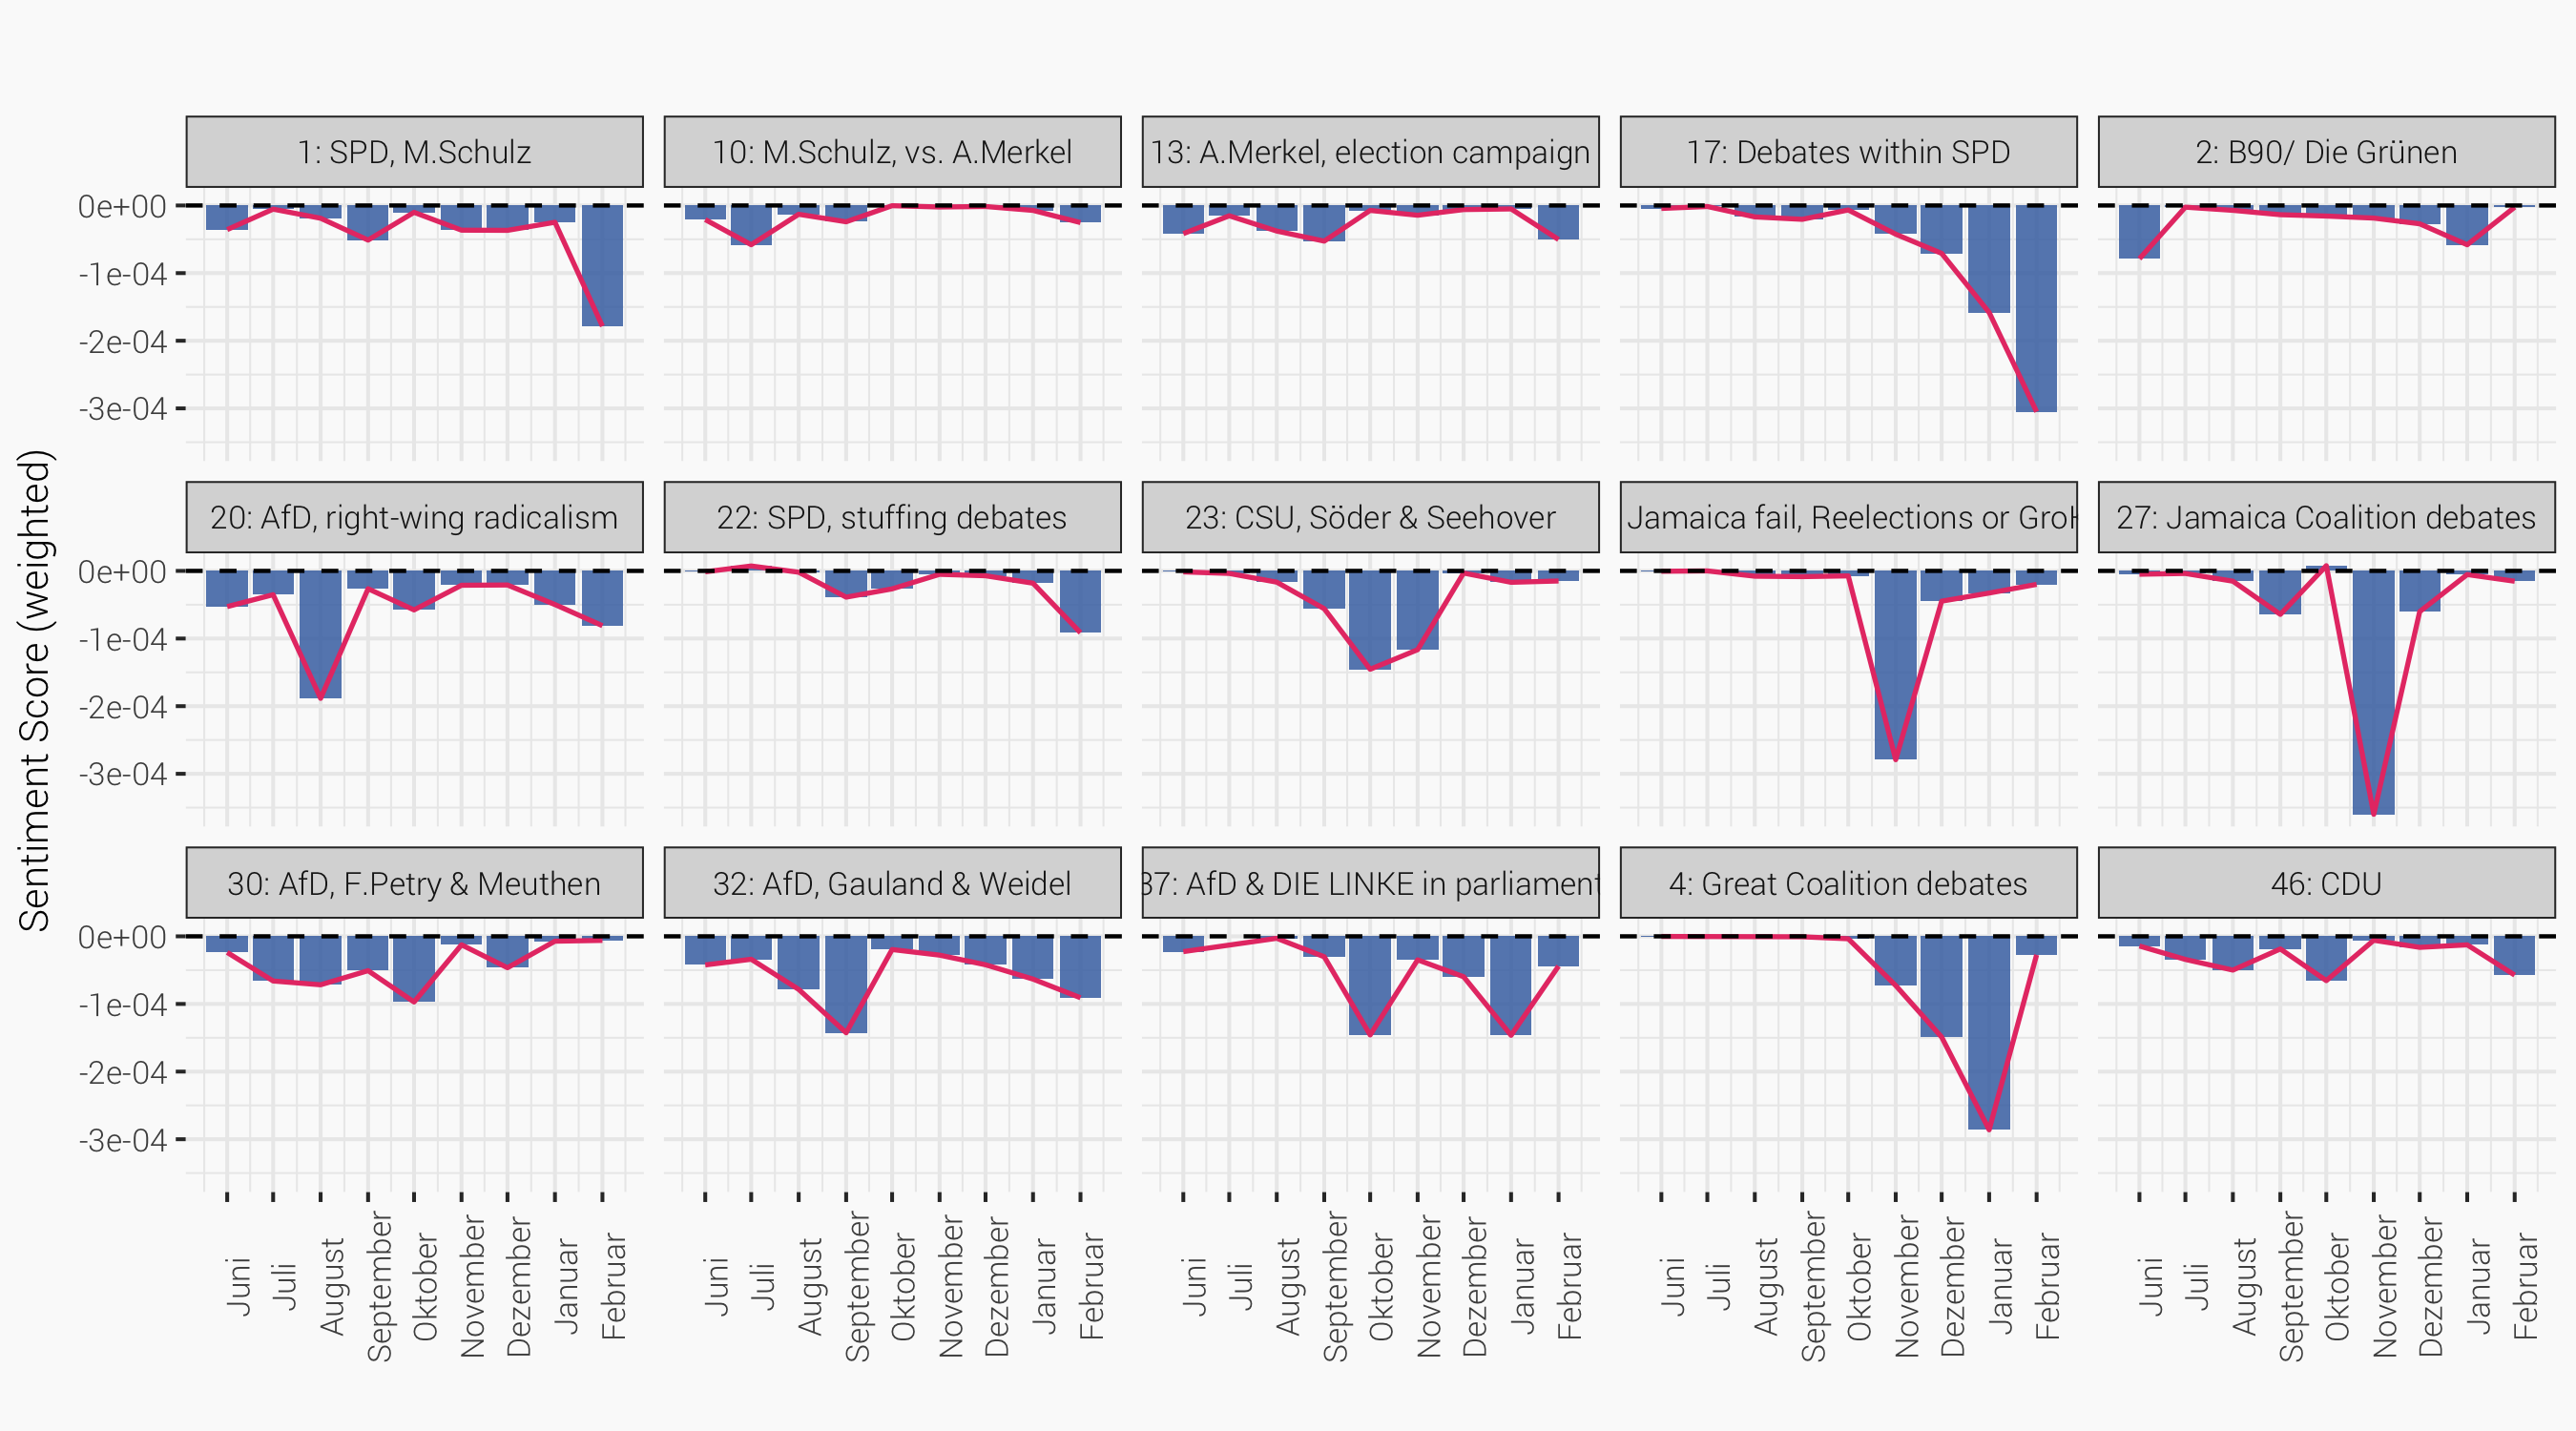
\includegraphics[width=\textwidth,keepaspectratio]{../figs/sentscore_monthly.png}
		\end{center}
	\label{fig_sentscore_monthly}
\end{figure}

In order to analyze the differences between the news websites, two different figures are considered: The bar plot is used to examine the polarity tendencies of the individual topics for a the respective website (Figure \ref{fig_sentscore_site}) and the radar plot is considered to observe the differences between the websites (Figure \ref{fig_sentscore_radar}).

Starting with the bar plot it becomes apparent that all topics are discussed negatively, except topic 23 at Tagesschau.de. At Bild.de, the topics that include the coalition negotiations (26, 27, 4) and the SPD (1, 17) are the most negative. The topics relating to AfD (20,30,32,37) are also discussed more negatively. Looking at the values of DIE WELT, two of the AfD topics have the most negative value (32, 20). Topic 27 concerning the Jamaica Coalition and the Grand Coalition (4) also score relatively negatively. Concerning FOCUS ONLINE, it is mainly topics that relate to the SPD (27, 17, 4, 1) that have a strong negative sentiment value, together with topic 32 and 37 - both related to AfD. Turning to SPIEGEL ONLINE, it is noticeable that the difference in sentiment value between the individual topics is less pronounced. Topics 13 (election campaign of A.Merkel) and 10 (A.Merkel vs M.Schulz) stand out as comparatively less negative. However, these issues are also the least negatively discussed in the other media. Also at stern.de the difference in sentiment value is less significant and overall less negative. The topics regarding CDU/CSU (46) and Martin Schulz (10) score the most positively (or least negatively). Tagesschau.de is the least negative on most topics, or even once positive. However, this does not apply to topic 23 (CSU), where tagesschau.de is most negative in comparison to the other media. As with Bild.de, the issues relating to the coalition negotiations (27 and 4) also come off rather badly with ZEIT ONLINE. However, the issues surrounding AfD (30, 32, 37 and 20) are even more negative than at Bild.de. 

\begin{figure}[H]
	\caption{Sentiment Score by news website}
	\begin{center}
			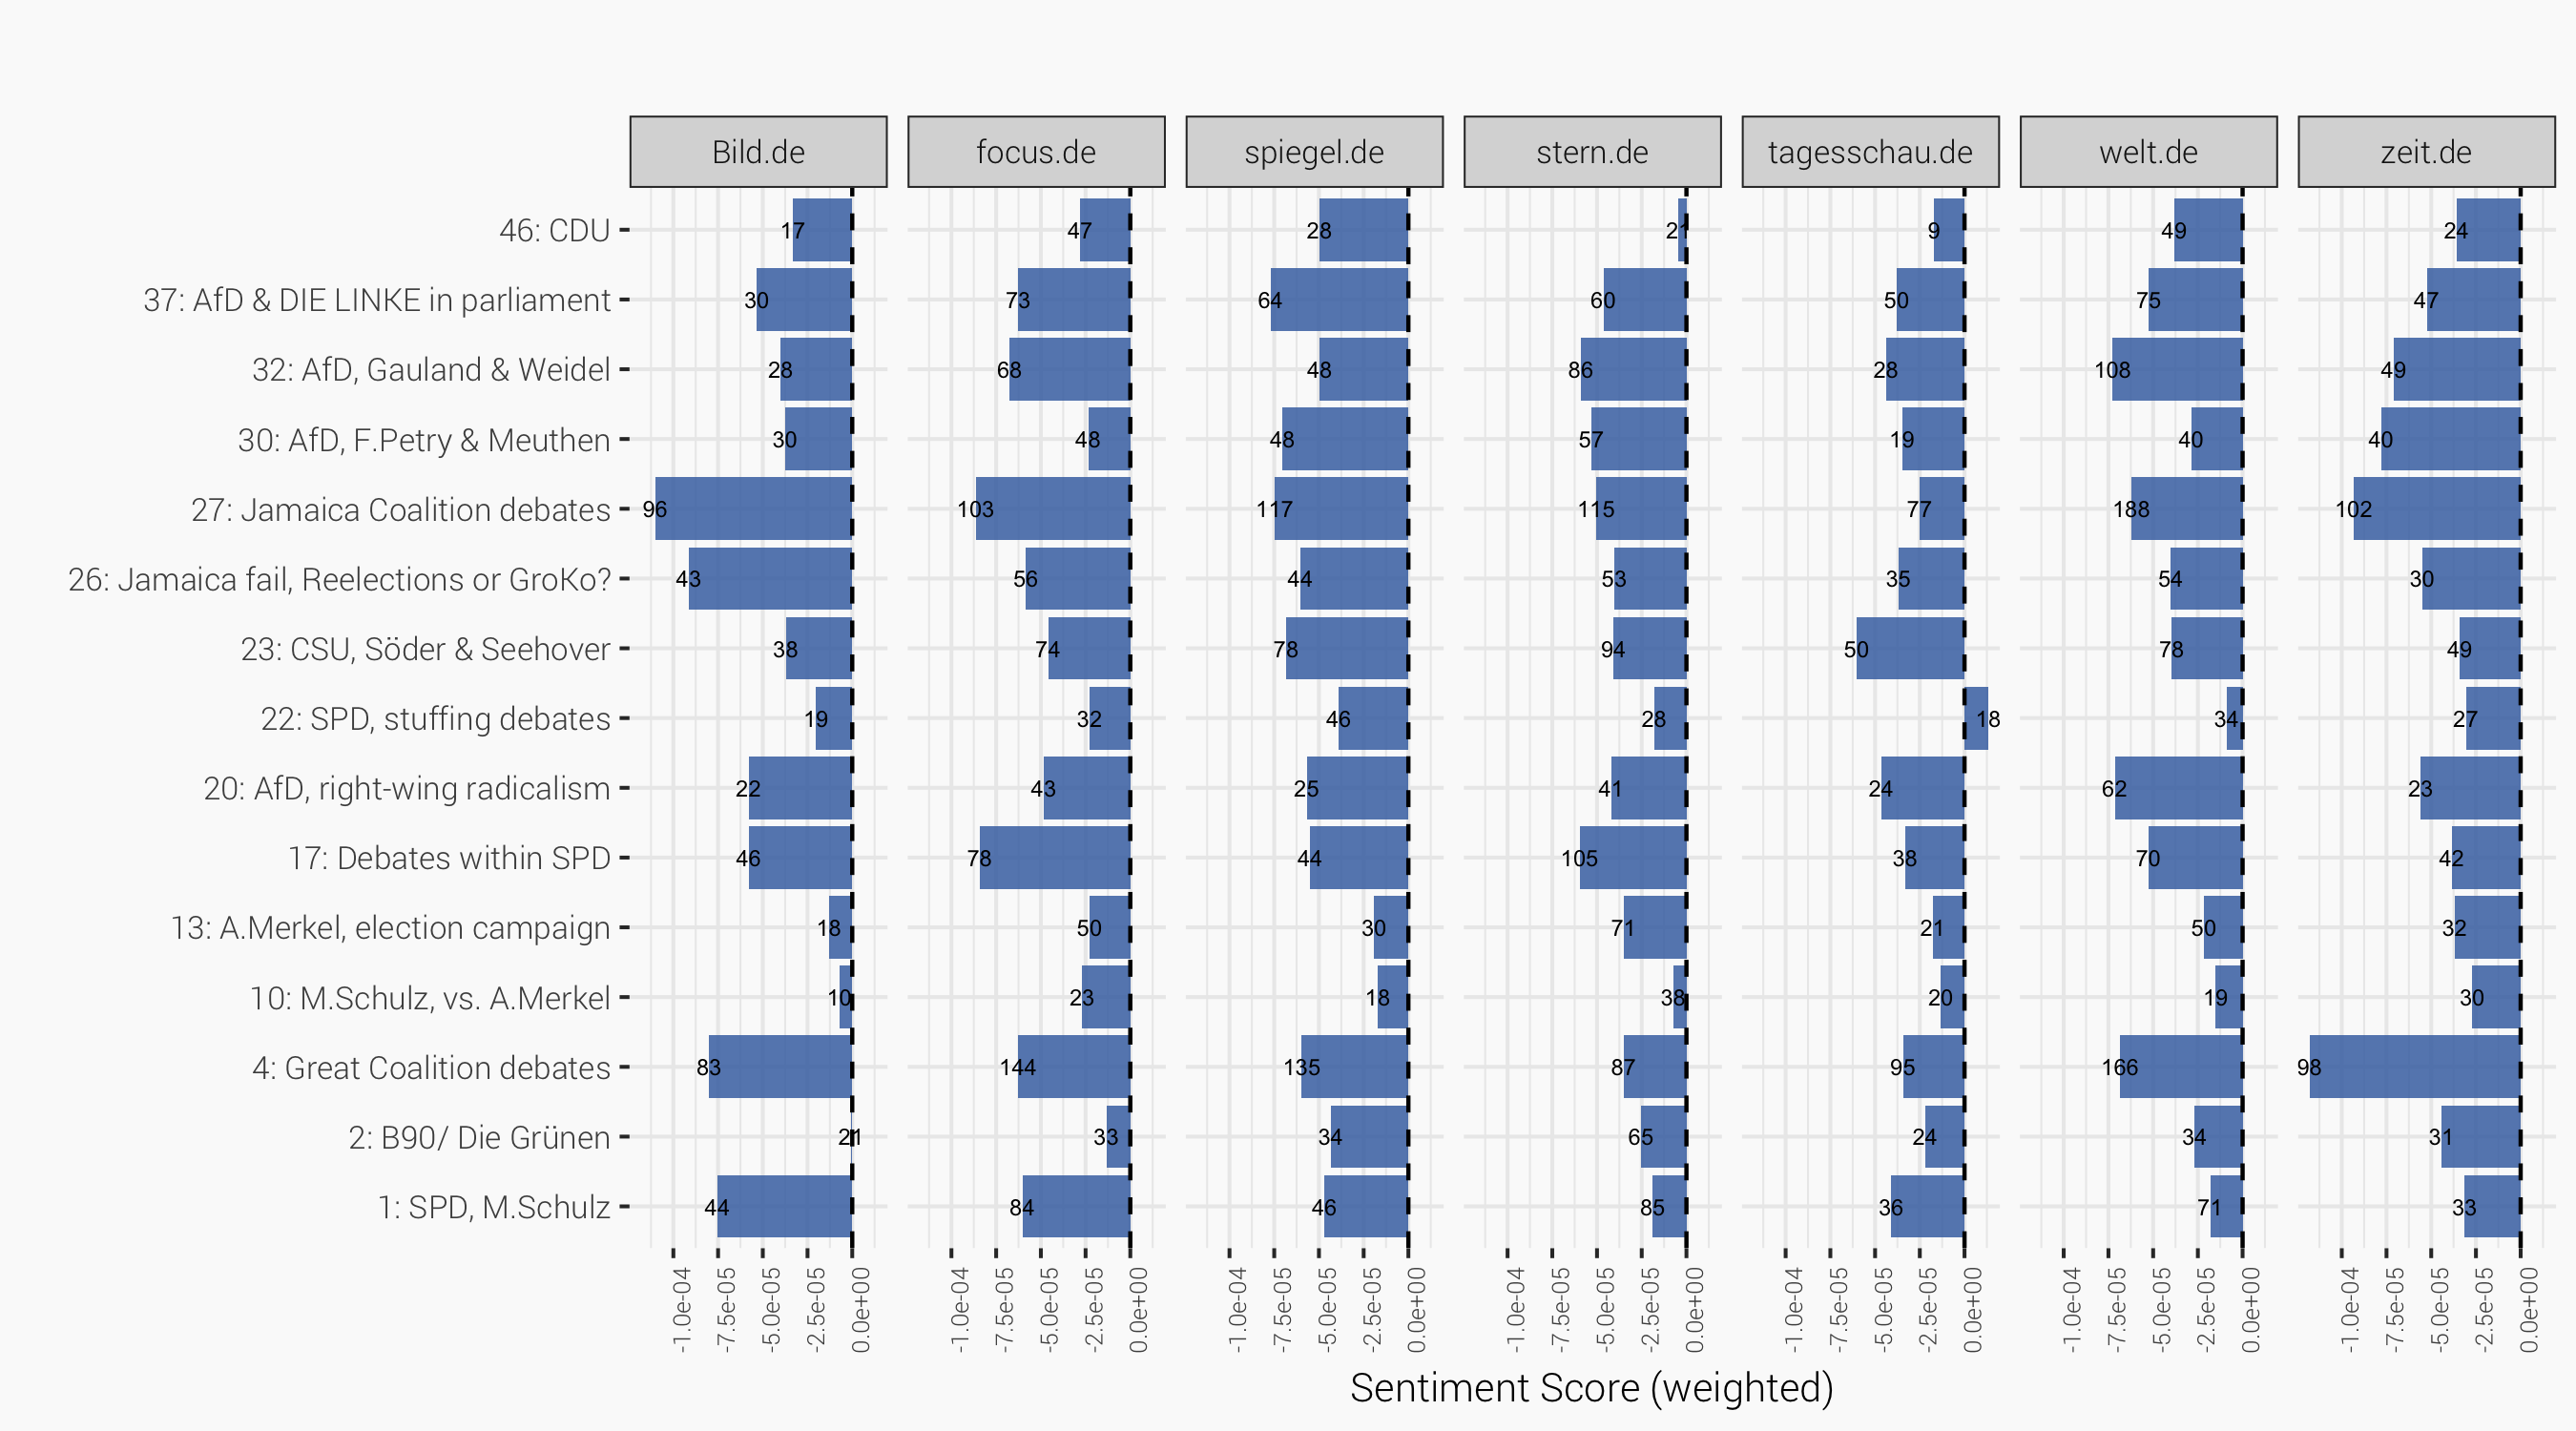
\includegraphics[width=\textwidth,keepaspectratio]{../figs/sentscore_site.png}
			\label{fig_sentscore_site}
	\end{center}
\end{figure}

A good overview of how differently the topics are discussed by the providers is shown in Figure \ref{fig_sentscore_radar}. It becomes evident that the sentiment value of the media differs most notably with regard to topic 27 and topic 4, i.e. the topics on which the coalition negotiations are reported. With regard to the Jamaica coalition, Bild.de reports the most and tagesschau.de the least negative. The reporting of ZEIT ONLINE concerning the grand coalition is the one with the most negative sentiment value and again Tagesschau.de, together with stern.de, the one with the value which is least negative. Furthermore, it becomes evident that the negative sentiment value of FOCUS ONLINE regarding topic 17 is high in relation to the other media. FOCUS ONLINE thus reports comparatively more negatively on the debates within the SPD. This includes in particular the vote on a possible coalition with CDU/CSU/CSU. For topic 1, which also deals with the SPD, the value of FOCUS ONLINE is rather negative, only undercut by Bild.de. Topics related to AfD do not show striking differences. 

\begin{figure}[H]
	\caption{Radar Plot of Sentiment Scores}
	\begin{center}
			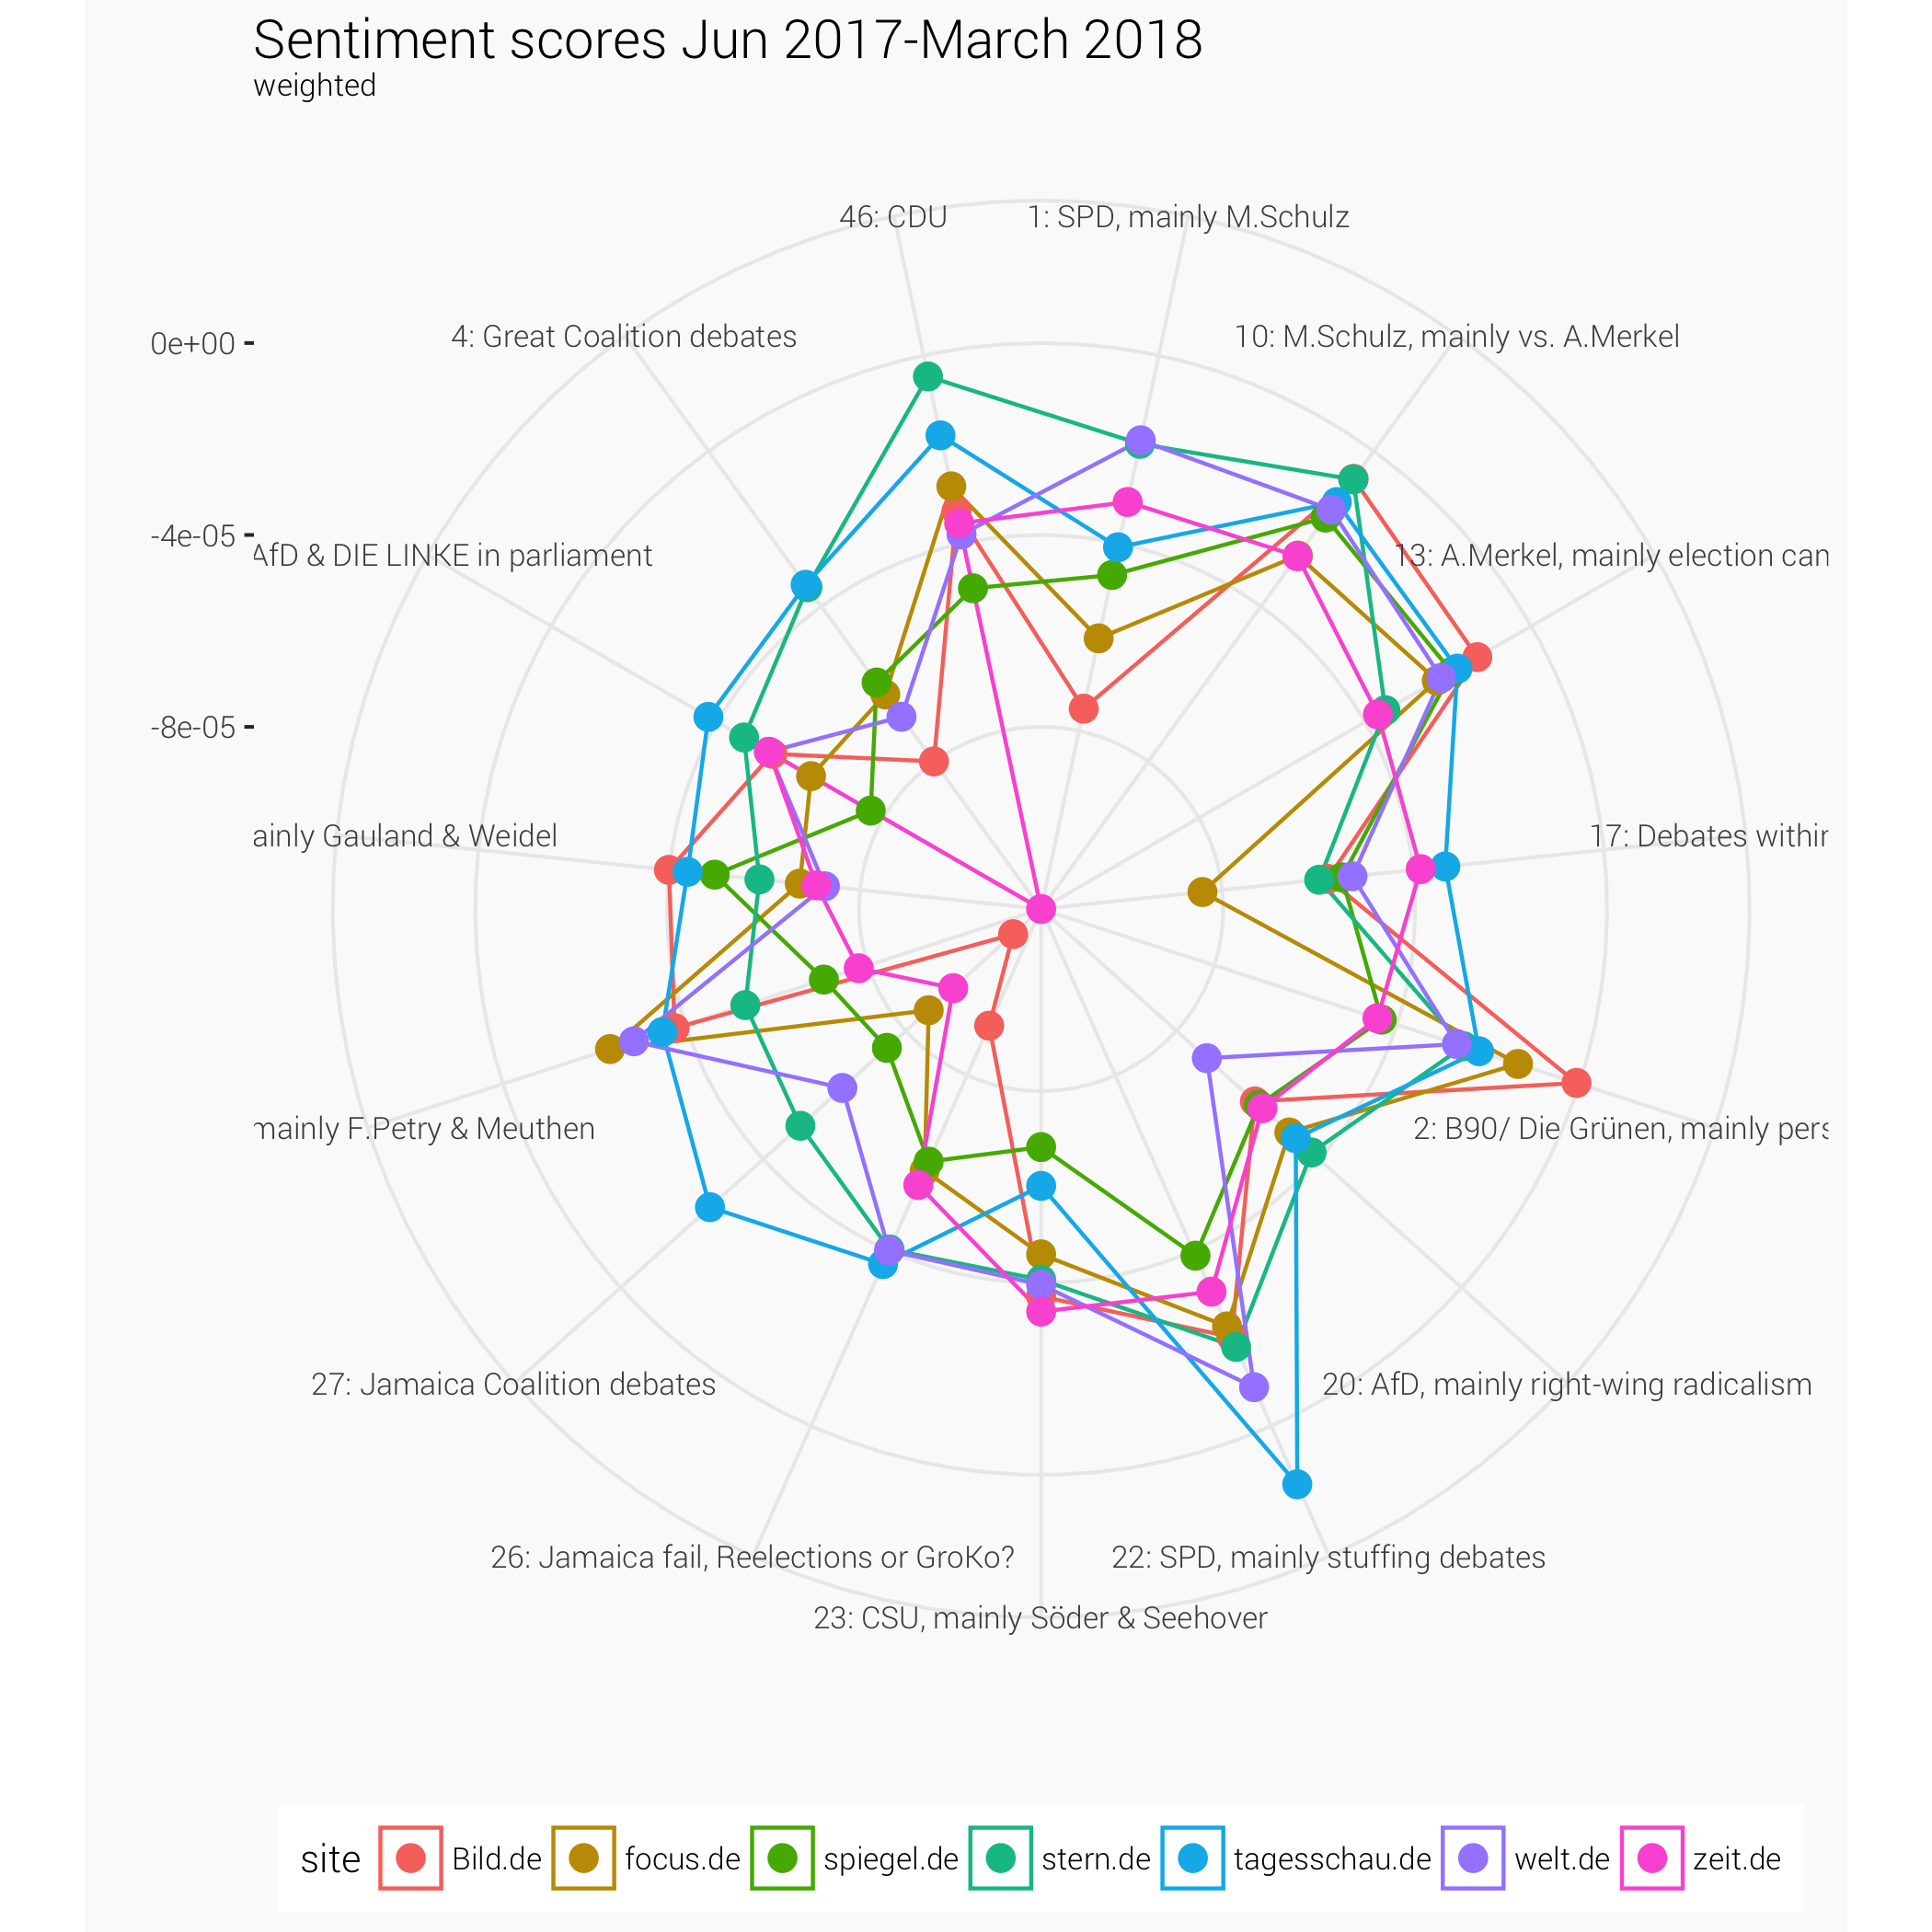
\includegraphics[width=0.8\textwidth,keepaspectratio]{../figs/sentscore_radar.png}
			\label{fig_sentscore_radar}
	\end{center}
\end{figure}

After the above figures have been analyzed, the following points can be summarized:

\begin{enumerate}
	\item The sentiment value of the SPD is decreasing over time, especially regarding debates within the party (topic 17). 
	\item The topics relating to the coalition talks on Jamaica (26, 27) and the grand coalition (4) are discussed rather critically, but they also show the greatest differences between the media. 
	\item In contrast, the tonality of the topics in relation to the AfD shows rather small differences. 
	\item Overall, the sentiment value at Tagesschau.de is the least negative and only shows a comparatively strong negative value at topic 23, concerning the CSU.
\end{enumerate} 

\subsection{News sentiment and poll data}\label{ch_correlation}

This section seeks to examine the association between sentiment reflected in online news content and phone survey poll results in Germany. Specifically, it aims to find the extent to which online sentiment and phone survey results correlate given a number of lags. I use the data from the "Sonntagsumfrage" (Sunday survey) from infratest dimap.\footnote{https://www.infratest-dimap.de/umfragen-analysen/bundesweit/sonntagsfrage/} The institution regularly asks at least 1000 German citizens the question: "Which party would you choose if federal elections take place next Sunday?" The survey thus measures the current election tendencies and therefore reflects an intermediate state in the opinion-forming process of the electoral population.

Much of the research on online content and political trends have focused on traditional weblogs and social media websites, such as Twitter, Facebook, MySpace, and YouTube. These studies have shown that social media is used to spread political opinions and that these considerations reflect the political landscape of the offline world. \citet{tumasjan_predicting_2010} investigate Tweets between August 13th and September 19th, 2009, prior to the German national elections to examine whether Twitter messages reflect the current offline political sentiment and whether it can be used to predict the popularity of parties or coalitions in the real world. With regard to the later question, they compare the share of attention the political parties receive on Twitter with the election result to examine whether the activity on Twitter can serve as a predictor of the election outcome. They found that the number of tweets reflects the election result and even comes close to traditional election polls.

\citet{fu_analyzing_2013} use a corpus of online posts from discussion forums and blogs to examine the extent to which online sentiment reflected in social media content can predict phone survey results in Hong Kong. They build a sentiment classifier conducting a support vector machine analysis on a training set of 2,000 manually labeled posts. In order to evaluate the temporal relationship between the time series of the online sentiment score and the results of the telephone survey, a cross correlation analysis was conducted, using the Box and Jenkins autoregressive integrated moving average (ARIMA) method \citep{box_time_2008}. Estimating the cross-correlation functions of the residuals, they find that online sentiment scores can lead phone survey results by about 8–15 days. 

In a more recent conference paper, \citet{padmaja_evaluating_2014} identify the scope of negation in news articles for two political parties in India (BJP and UPA) to analyze how the choice of certain words used in these texts influence the sentiments of public in polls. Comparing three different sentiment analysis methods (two machine learning and one dictionary method), they observe that the choice of certain words used in political text was influencing the sentiments in favor of BJP. They conclude that this sentiment bias might be one of the causes for the election results in 2014.

In the present paper, the relationship between monthly average of both the sentiment value of individual topics ($x_t$) and the survey value of the parties ($y_t$) is estimated using the cross correlation function (CCF). Thus, the CCF between $x_{t+h}$ and $y_t$ for $h\pm 1$,$h \pm 2$,$h \pm 3$ is computed. A negative value for $h$ is a correlation between the topic sentiment value at a time before $t$ and the survey value at time $t$. The correlation value for $h=0$ indicates the contemporary correlation between the two time series.  Based on the coefficients of the cross correlation estimation shown in Figure \ref{fig_ccf}, the significant correlations between topic sentiment and survey value are evaluated for each party.\footnote{The value of the cross correlation coefficients for lag 0 can be found in the Appendix (Table \ref{apx_corr})} It is important to note that no causal relationships are described below, but that only the correlation between the two time series is described. 

The survey results of the AfD correlate negatively with topics relating to the SPD (17, 22) at lag 0. Thus, if the SPD was more negatively reported, the poll value of the AfD increased in the same month (and vice versa). Another significant negative correlation exists between the reporting on the GroKo (4) and the survey value of AfD at lag -1 ($x_{t-1}$). So if the GroKo was more negatively reported in one month, the survey value of the AfD increased in the following month (and vice versa). For the FDP, too, only negative correlation coefficients can be detected, with the strongest negative correlation existing for the topic relating to the CSU (23). If the CSU got off worse in the online news, the poll value of the FDP have gone up. Another interesting observation is that the FDP's poll results correlate negatively with issues relating to the Jamaica coalition at lag 1 ($x_{t+1}$). So if the poll results for the FDP rose in one month, the following month the FDP was reported more negatively. The Green Party survey results show no negative correlation with any of the topics, except topic 30 at lag 1. It is striking that there seems to be a strong negative correlation between the SPD topics (1, 17, 22) and the poll results of the left party (DIE LINKE). This means that the poll value of the left party has climbed if the topics related to the SPD were discussed more negatively. Same applies to the reporting on the GroKo (30) for lag -1. Conversely, the SPD's survey results correlate strongly positively with these topics, and also with topic 30 with a delay of one month. For the CDU/CSU, too, only significant negative correlations are discernible: the survey results correlate negatively with the topic of the Schulz v Merkel debate (10) and negatively with topic 30 with a delay of one month ($x_{t+1}$). 

\begin{figure}[H]
	\caption{Cross-Correlation}
	\begin{center}
			\includegraphics[width=\textwidth,keepaspectratio]{../figs/ccf2.png}
			\label{fig_ccf}
	\end{center}
\end{figure} 

After the above figure have been analyzed, the following points can be summarized:

\begin{enumerate}
	\item Only the survey results of the SPD correlate positively with the emotional value of the topics. There seems to be a strong correlation between the way topics concerning the SPD are discussed in the online news and the poll results.  
	\item The poll results of the Left Party, on the other hand, seem to correlate negatively with the reporting on the SPD. 
	\item Similar tendencies can also be seen with regard to the AfD, since here too the survey results correlate significantly negatively with the topics about the SPD and the grand coalition. 
\end{enumerate} 

Summarizing the analyses from this and the previous section, it can be observed that the positive correlation between the emotional value of the reporting and the survey value of a party is particularly large if the reporting is conspicuously negative. 

\section{Conclusion}

The purpose of this paper was to examine (1) whether the political reporting of different media differs in terms of topic frequency and topic tonality and (2) whether this reporting correlates with the opinion-forming process of the voters. Regarding (1) the analysis revealed that there are differences between the media considered, both in terms of topic prevalence and the way in which these topics are discussed. Although overall all topics are discussed negatively, there are still differences, especially regarding the coalition negotiations. The smallest differences can be found for topic concerning the AfD. With regard to (2), the analysis has shown that the tonality of topics discussed by the SPD shows a strong positive correlation to current survey results. Overall, there seems to be a link between reporting on political issues and electoral preferences. Further research should focus on the exact causal relationships between these two concepts. 

\pagebreak

\printbibliography

\appendix
\section{Appendices}

\subsection{Most frequent words}\label{apx_tf}
% 1, 2
\begin{figure}[H]
	\begin{center}
		\begin{subfigure}[normla]{0.49\textwidth}
			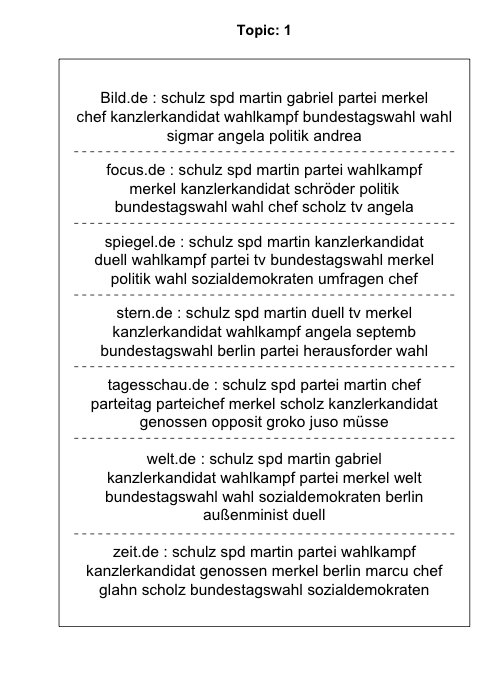
\includegraphics[width=\textwidth]{../figs/plotquote1.png}
		\end{subfigure}
		\begin{subfigure}[normla]{0.49\textwidth}
			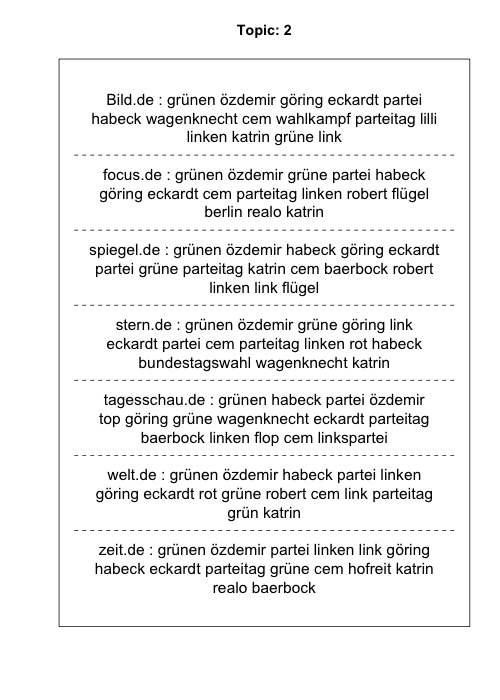
\includegraphics[width=\textwidth]{../figs/plotquote2.png}
		\end{subfigure}
	\end{center}
\end{figure}
	
% 4, 10
\begin{figure}[H]
	\begin{center}
		\begin{subfigure}[normla]{0.49\textwidth}
			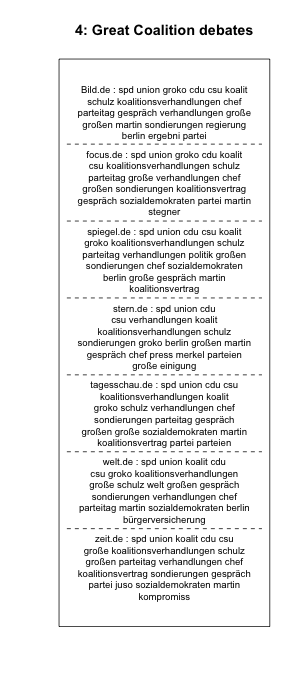
\includegraphics[width=\textwidth]{../figs/plotquote4.png}
		\end{subfigure}
		\begin{subfigure}[normla]{0.49\textwidth}
			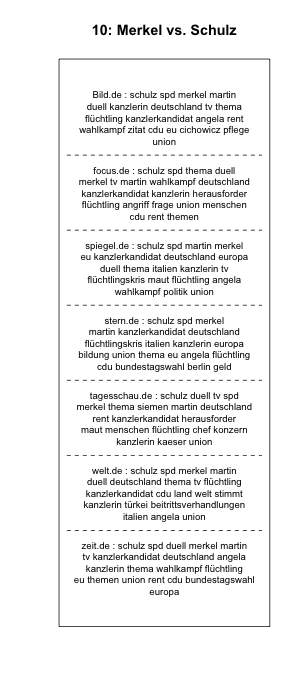
\includegraphics[width=\textwidth]{../figs/plotquote10.png}
		\end{subfigure}
	\end{center}
\end{figure}

% 13, 17
\begin{figure}[H]
	\begin{center}
		\begin{subfigure}[normla]{0.49\textwidth}
			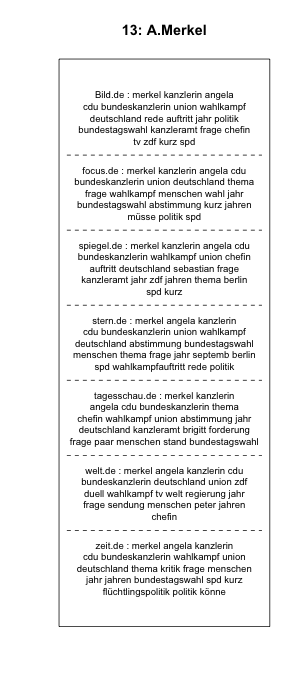
\includegraphics[width=\textwidth]{../figs/plotquote13.png}
		\end{subfigure}
		\begin{subfigure}[normla]{0.49\textwidth}
			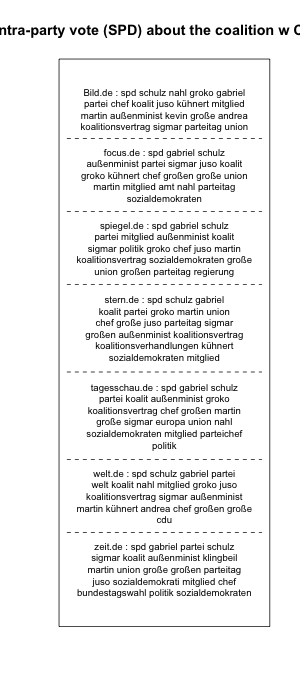
\includegraphics[width=\textwidth]{../figs/plotquote17.png}
		\end{subfigure}
	\end{center}
\end{figure}

% 20, 23
\begin{figure}[H]
	\begin{center}
		\begin{subfigure}[normla]{0.49\textwidth}
			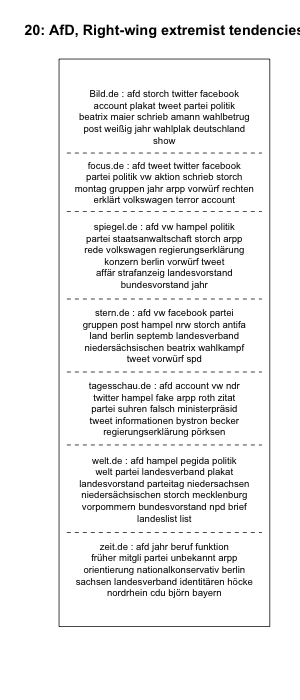
\includegraphics[width=\textwidth]{../figs/plotquote20.png}
		\end{subfigure}
		\begin{subfigure}[normla]{0.49\textwidth}
			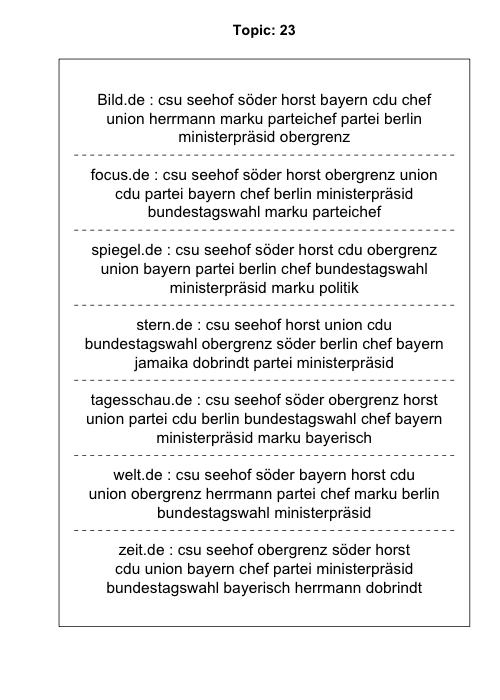
\includegraphics[width=\textwidth]{../figs/plotquote23.png}
		\end{subfigure}
	\end{center}
\end{figure}

% 26, 27
\begin{figure}[H]
	\begin{center}
		\begin{subfigure}[normla]{0.49\textwidth}
			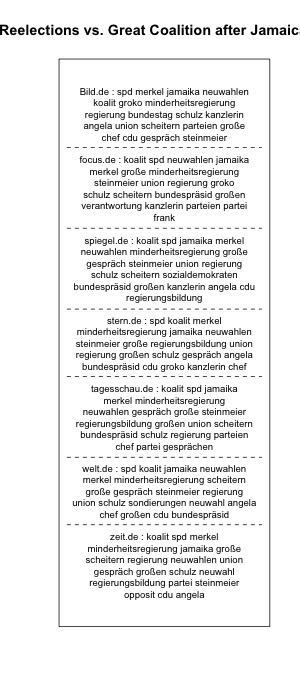
\includegraphics[width=\textwidth]{../figs/plotquote26.png}
		\end{subfigure}
		\begin{subfigure}[normla]{0.49\textwidth}
			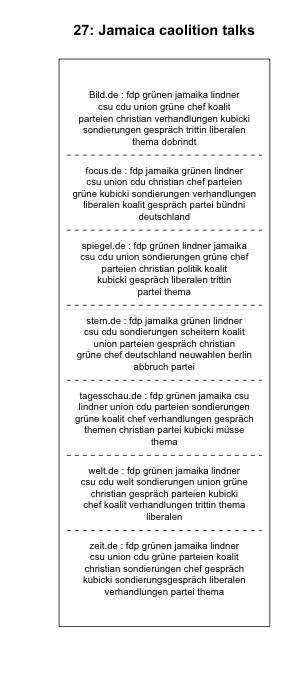
\includegraphics[width=\textwidth]{../figs/plotquote27.png}
		\end{subfigure}
	\end{center}
\end{figure}

% 30, 32
\begin{figure}[H]
	\begin{center}
		\begin{subfigure}[normla]{0.49\textwidth}
			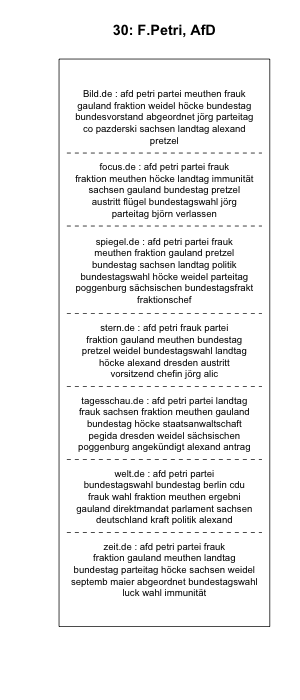
\includegraphics[width=\textwidth]{../figs/plotquote30.png}
		\end{subfigure}
		\begin{subfigure}[normla]{0.49\textwidth}
			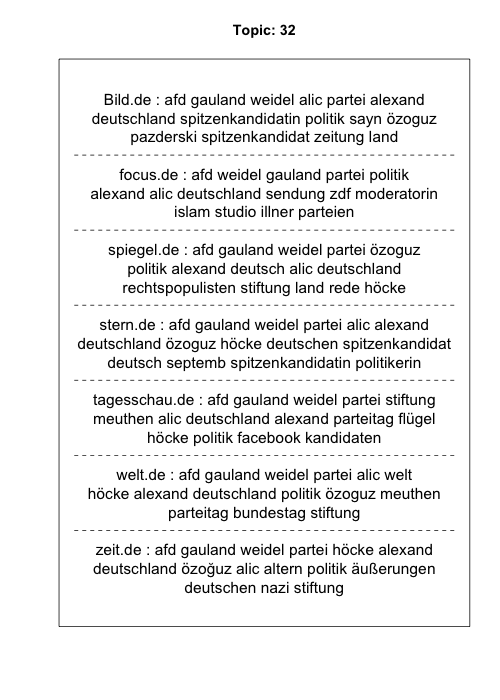
\includegraphics[width=\textwidth]{../figs/plotquote32.png}
		\end{subfigure}
	\end{center}
\end{figure}

% 37, 46
\begin{figure}[H]
	\begin{center}
		\begin{subfigure}[normla]{0.49\textwidth}
			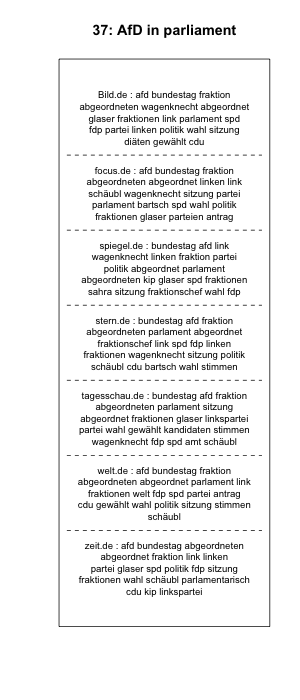
\includegraphics[width=\textwidth]{../figs/plotquote37.png}
		\end{subfigure}
		\begin{subfigure}[normla]{0.49\textwidth}
			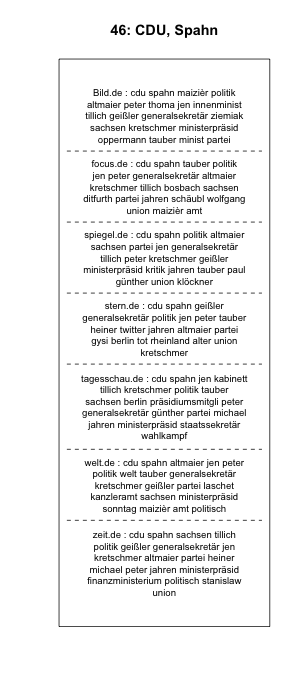
\includegraphics[width=\textwidth]{../figs/plotquote46.png}
		\end{subfigure}
	\end{center}
\end{figure}

\subsection{Regression Results}\label{apx_coeff}
% latex table generated in R 3.4.2 by xtable 1.8-2 package
% Mon Apr  9 18:06:43 2018
\begin{table}[ht]
\centering
\resizebox{\textwidth}{!}{
\begin{tabular}{rllrrrr}
  \hline
 & topic\_name & parameter & Estimate & Std. Error & t value & p \\ 
  \hline
1 & 1: SPD, M.Schulz & (Intercept) & 0.04 & 0.00 & 11.50 & 0.00 \\ 
  2 & 1: SPD, M.Schulz & FOCUS ONLINE & -0.01 & 0.00 & -2.04 & 0.04 \\ 
  3 & 1: SPD, M.Schulz & SPIEGEL ONLINE & -0.01 & 0.00 & -1.88 & 0.06 \\ 
  4 & 1: SPD, M.Schulz & stern.de & -0.01 & 0.00 & -2.48 & 0.01 \\ 
  5 & 1: SPD, M.Schulz & Tagesschau.de & -0.02 & 0.00 & -3.42 & 0.00 \\ 
  6 & 1: SPD, M.Schulz & DIE WELT & -0.01 & 0.00 & -3.83 & 0.00 \\ 
  7 & 1: SPD, M.Schulz & ZEIT ONLINE & -0.01 & 0.00 & -2.76 & 0.01 \\ 
  8 & 2: B90/ Die Grünen & (Intercept) & 0.02 & 0.00 & 6.42 & 0.00 \\ 
  9 & 2: B90/ Die Grünen & FOCUS ONLINE & -0.01 & 0.00 & -1.46 & 0.14 \\ 
  10 & 2: B90/ Die Grünen & SPIEGEL ONLINE & 0.00 & 0.00 & 0.29 & 0.77 \\ 
  11 & 2: B90/ Die Grünen & stern.de & 0.01 & 0.00 & 1.61 & 0.11 \\ 
  12 & 2: B90/ Die Grünen & Tagesschau.de & -0.00 & 0.00 & -0.72 & 0.47 \\ 
  13 & 2: B90/ Die Grünen & DIE WELT & -0.00 & 0.00 & -1.12 & 0.26 \\ 
  14 & 2: B90/ Die Grünen & ZEIT ONLINE & 0.00 & 0.00 & 1.03 & 0.30 \\ 
  15 & 4: Great Coalition debates & (Intercept) & 0.06 & 0.00 & 13.48 & 0.00 \\ 
  16 & 4: Great Coalition debates & FOCUS ONLINE & -0.01 & 0.01 & -1.85 & 0.06 \\ 
  17 & 4: Great Coalition debates & SPIEGEL ONLINE & 0.00 & 0.01 & 0.33 & 0.74 \\ 
  18 & 4: Great Coalition debates & stern.de & -0.03 & 0.01 & -5.76 & 0.00 \\ 
  19 & 4: Great Coalition debates & Tagesschau.de & -0.01 & 0.01 & -0.93 & 0.35 \\ 
  20 & 4: Great Coalition debates & DIE WELT & -0.01 & 0.01 & -2.39 & 0.02 \\ 
  21 & 4: Great Coalition debates & ZEIT ONLINE & 0.00 & 0.01 & 0.20 & 0.84 \\ 
  22 & 10: M.Schulz, vs. A.Merkel & (Intercept) & 0.01 & 0.00 & 3.85 & 0.00 \\ 
  23 & 10: M.Schulz, vs. A.Merkel & FOCUS ONLINE & 0.00 & 0.00 & 0.18 & 0.86 \\ 
  24 & 10: M.Schulz, vs. A.Merkel & SPIEGEL ONLINE & 0.00 & 0.00 & 0.54 & 0.59 \\ 
  25 & 10: M.Schulz, vs. A.Merkel & stern.de & 0.01 & 0.00 & 2.57 & 0.01 \\ 
  26 & 10: M.Schulz, vs. A.Merkel & Tagesschau.de & 0.00 & 0.00 & 0.87 & 0.38 \\ 
  27 & 10: M.Schulz, vs. A.Merkel & DIE WELT & -0.00 & 0.00 & -1.10 & 0.27 \\ 
  28 & 10: M.Schulz, vs. A.Merkel & ZEIT ONLINE & 0.01 & 0.00 & 3.60 & 0.00 \\ 
  29 & 13: A.Merkel, election campaign & (Intercept) & 0.02 & 0.00 & 9.27 & 0.00 \\ 
  30 & 13: A.Merkel, election campaign & FOCUS ONLINE & 0.00 & 0.00 & 0.47 & 0.64 \\ 
  31 & 13: A.Merkel, election campaign & SPIEGEL ONLINE & 0.00 & 0.00 & 0.92 & 0.36 \\ 
  32 & 13: A.Merkel, election campaign & stern.de & 0.01 & 0.00 & 2.72 & 0.01 \\ 
  33 & 13: A.Merkel, election campaign & Tagesschau.de & -0.01 & 0.00 & -1.58 & 0.11 \\ 
  34 & 13: A.Merkel, election campaign & DIE WELT & 0.00 & 0.00 & 0.33 & 0.74 \\ 
  35 & 13: A.Merkel, election campaign & ZEIT ONLINE & 0.00 & 0.00 & 1.19 & 0.23 \\ 
  36 & 17: Debates within SPD & (Intercept) & 0.04 & 0.00 & 10.16 & 0.00 \\ 
  37 & 17: Debates within SPD & FOCUS ONLINE & -0.01 & 0.00 & -1.31 & 0.19 \\ 
  38 & 17: Debates within SPD & SPIEGEL ONLINE & -0.01 & 0.00 & -2.17 & 0.03 \\ 
  39 & 17: Debates within SPD & stern.de & -0.00 & 0.00 & -0.42 & 0.67 \\ 
  40 & 17: Debates within SPD & Tagesschau.de & -0.01 & 0.00 & -3.00 & 0.00 \\ 
  41 & 17: Debates within SPD & DIE WELT & -0.01 & 0.00 & -2.69 & 0.01 \\ 
  42 & 17: Debates within SPD & ZEIT ONLINE & -0.01 & 0.00 & -1.74 & 0.08 \\ 
  43 & 20: AfD, right-wing radicalism & (Intercept) & 0.02 & 0.00 & 6.25 & 0.00 \\ 
  44 & 20: AfD, right-wing radicalism & FOCUS ONLINE & -0.00 & 0.00 & -0.68 & 0.49 \\ 
  45 & 20: AfD, right-wing radicalism & SPIEGEL ONLINE & -0.00 & 0.00 & -0.80 & 0.42 \\ 
  46 & 20: AfD, right-wing radicalism & stern.de & -0.00 & 0.00 & -0.90 & 0.37 \\ 
  47 & 20: AfD, right-wing radicalism & Tagesschau.de & -0.00 & 0.00 & -0.03 & 0.98 \\ 
  48 & 20: AfD, right-wing radicalism & DIE WELT & 0.00 & 0.00 & 0.49 & 0.62 \\ 
  49 & 20: AfD, right-wing radicalism & ZEIT ONLINE & -0.00 & 0.00 & -0.57 & 0.57 \\ 
  50 & 22: SPD, stuffing debates & (Intercept) & 0.02 & 0.00 & 7.05 & 0.00 \\ 
  51 & 22: SPD, stuffing debates & FOCUS ONLINE & -0.00 & 0.00 & -1.08 & 0.28 \\ 
  52 & 22: SPD, stuffing debates & SPIEGEL ONLINE & 0.01 & 0.00 & 3.09 & 0.00 \\ 
  53 & 22: SPD, stuffing debates & stern.de & -0.01 & 0.00 & -1.98 & 0.05 \\ 
  54 & 22: SPD, stuffing debates & Tagesschau.de & -0.00 & 0.00 & -0.91 & 0.36 \\ 
  55 & 22: SPD, stuffing debates & DIE WELT & -0.00 & 0.00 & -1.23 & 0.22 \\ 
  56 & 22: SPD, stuffing debates & ZEIT ONLINE & 0.01 & 0.00 & 1.43 & 0.15 \\ 
   \hline
\end{tabular}
}
\end{table}

% latex table generated in R 3.4.2 by xtable 1.8-2 package
% Mon Apr  9 18:06:44 2018
\begin{table}[ht]
\centering
\resizebox{\textwidth}{!}{
\begin{tabular}{rllrrrr}
  \hline
 & topic\_name & parameter & Estimate & Std. Error & t value & p \\ 
  \hline
57 & 23: CSU, Söder \& Seehover & (Intercept) & 0.04 & 0.00 & 9.36 & 0.00 \\ 
  58 & 23: CSU, Söder \& Seehover & FOCUS ONLINE & -0.00 & 0.00 & -0.74 & 0.46 \\ 
  59 & 23: CSU, Söder \& Seehover & SPIEGEL ONLINE & 0.01 & 0.00 & 1.29 & 0.20 \\ 
  60 & 23: CSU, Söder \& Seehover & stern.de & -0.00 & 0.00 & -0.36 & 0.72 \\ 
  61 & 23: CSU, Söder \& Seehover & Tagesschau.de & -0.01 & 0.01 & -1.13 & 0.26 \\ 
  62 & 23: CSU, Söder \& Seehover & DIE WELT & -0.01 & 0.00 & -1.16 & 0.25 \\ 
  63 & 23: CSU, Söder \& Seehover & ZEIT ONLINE & 0.00 & 0.01 & 0.44 & 0.66 \\ 
  64 & 26: Jamaica fail, Reelections or GroKo? & (Intercept) & 0.03 & 0.00 & 12.15 & 0.00 \\ 
  65 & 26: Jamaica fail, Reelections or GroKo? & FOCUS ONLINE & -0.00 & 0.00 & -1.17 & 0.24 \\ 
  66 & 26: Jamaica fail, Reelections or GroKo? & SPIEGEL ONLINE & -0.00 & 0.00 & -1.12 & 0.26 \\ 
  67 & 26: Jamaica fail, Reelections or GroKo? & stern.de & -0.01 & 0.00 & -3.56 & 0.00 \\ 
  68 & 26: Jamaica fail, Reelections or GroKo? & Tagesschau.de & -0.01 & 0.00 & -2.61 & 0.01 \\ 
  69 & 26: Jamaica fail, Reelections or GroKo? & DIE WELT & -0.01 & 0.00 & -3.37 & 0.00 \\ 
  70 & 26: Jamaica fail, Reelections or GroKo? & ZEIT ONLINE & -0.01 & 0.00 & -1.44 & 0.15 \\ 
  71 & 27: Jamaica Coalition debates & (Intercept) & 0.07 & 0.00 & 14.34 & 0.00 \\ 
  72 & 27: Jamaica Coalition debates & FOCUS ONLINE & -0.03 & 0.01 & -5.20 & 0.00 \\ 
  73 & 27: Jamaica Coalition debates & SPIEGEL ONLINE & -0.01 & 0.01 & -1.40 & 0.16 \\ 
  74 & 27: Jamaica Coalition debates & stern.de & -0.03 & 0.01 & -5.13 & 0.00 \\ 
  75 & 27: Jamaica Coalition debates & Tagesschau.de & -0.02 & 0.01 & -2.75 & 0.01 \\ 
  76 & 27: Jamaica Coalition debates & DIE WELT & -0.01 & 0.01 & -1.38 & 0.17 \\ 
  77 & 27: Jamaica Coalition debates & ZEIT ONLINE & -0.00 & 0.01 & -0.51 & 0.61 \\ 
  78 & 30: AfD, F.Petry \& Meuthen & (Intercept) & 0.03 & 0.00 & 7.87 & 0.00 \\ 
  79 & 30: AfD, F.Petry \& Meuthen & FOCUS ONLINE & -0.00 & 0.00 & -1.25 & 0.21 \\ 
  80 & 30: AfD, F.Petry \& Meuthen & SPIEGEL ONLINE & 0.00 & 0.00 & 0.49 & 0.62 \\ 
  81 & 30: AfD, F.Petry \& Meuthen & stern.de & -0.00 & 0.00 & -0.95 & 0.34 \\ 
  82 & 30: AfD, F.Petry \& Meuthen & Tagesschau.de & -0.01 & 0.00 & -3.23 & 0.00 \\ 
  83 & 30: AfD, F.Petry \& Meuthen & DIE WELT & -0.01 & 0.00 & -2.64 & 0.01 \\ 
  84 & 30: AfD, F.Petry \& Meuthen & ZEIT ONLINE & 0.00 & 0.00 & 0.92 & 0.36 \\ 
  85 & 32: AfD, Gauland \& Weidel & (Intercept) & 0.02 & 0.00 & 6.84 & 0.00 \\ 
  86 & 32: AfD, Gauland \& Weidel & FOCUS ONLINE & 0.00 & 0.00 & 0.14 & 0.89 \\ 
  87 & 32: AfD, Gauland \& Weidel & SPIEGEL ONLINE & -0.00 & 0.00 & -0.17 & 0.86 \\ 
  88 & 32: AfD, Gauland \& Weidel & stern.de & 0.01 & 0.00 & 1.63 & 0.10 \\ 
  89 & 32: AfD, Gauland \& Weidel & Tagesschau.de & -0.01 & 0.00 & -1.37 & 0.17 \\ 
  90 & 32: AfD, Gauland \& Weidel & DIE WELT & 0.01 & 0.00 & 1.49 & 0.14 \\ 
  91 & 32: AfD, Gauland \& Weidel & ZEIT ONLINE & 0.01 & 0.00 & 1.25 & 0.21 \\ 
  92 & 37: AfD \& DIE LINKE in parliament & (Intercept) & 0.02 & 0.00 & 7.01 & 0.00 \\ 
  93 & 37: AfD \& DIE LINKE in parliament & FOCUS ONLINE & 0.01 & 0.00 & 1.16 & 0.25 \\ 
  94 & 37: AfD \& DIE LINKE in parliament & SPIEGEL ONLINE & 0.01 & 0.00 & 2.83 & 0.00 \\ 
  95 & 37: AfD \& DIE LINKE in parliament & stern.de & 0.00 & 0.00 & 0.19 & 0.85 \\ 
  96 & 37: AfD \& DIE LINKE in parliament & Tagesschau.de & 0.01 & 0.00 & 1.09 & 0.28 \\ 
  97 & 37: AfD \& DIE LINKE in parliament & DIE WELT & 0.00 & 0.00 & 0.37 & 0.71 \\ 
  98 & 37: AfD \& DIE LINKE in parliament & ZEIT ONLINE & 0.01 & 0.00 & 2.13 & 0.03 \\ 
  99 & 46: CDU & (Intercept) & 0.02 & 0.00 & 7.35 & 0.00 \\ 
  100 & 46: CDU & FOCUS ONLINE & -0.00 & 0.00 & -0.32 & 0.75 \\ 
  101 & 46: CDU & SPIEGEL ONLINE & 0.00 & 0.00 & 0.71 & 0.48 \\ 
  102 & 46: CDU & stern.de & -0.01 & 0.00 & -1.98 & 0.05 \\ 
  103 & 46: CDU & Tagesschau.de & -0.01 & 0.00 & -3.37 & 0.00 \\ 
  104 & 46: CDU & DIE WELT & -0.00 & 0.00 & -0.52 & 0.60 \\ 
  105 & 46: CDU & ZEIT ONLINE & -0.00 & 0.00 & -0.08 & 0.93 \\ 
   \hline
\end{tabular}
}
\end{table}


\subsection{Cross Correlation Coefficient}
% latex table generated in R 3.4.2 by xtable 1.8-2 package
% Sun May  6 21:05:39 2018
\begin{table}[ht]
\centering
\begin{adjustbox}{width=\textwidth}
\begin{tabular}{rlrrrrrr}
  \hline
 & Var1 & AfD & FDP & Grüne & Linke & SPD & Union \\ 
  \hline
1 & 1: SPD, M.Schulz & -0.636 & 0.072 & -0.438 & -0.693 & 0.752 & 0.199 \\ 
  2 & 10: M.Schulz, vs. A.Merkel & 0.438 & 0.566 & 0.505 & 0.341 & -0.229 & -0.758 \\ 
  3 & 13: A.Merkel, election campaign & 0.098 & 0.350 & 0.440 & -0.060 & 0.076 & -0.507 \\ 
  4 & 17: Debates within SPD & -0.770 & 0.075 & -0.676 & -0.754 & 0.841 & 0.382 \\ 
  5 & 2: B90/ Die Grünen & 0.253 & -0.092 & 0.185 & 0.480 & -0.329 & -0.048 \\ 
  6 & 20: AfD, right-wing radicalism & 0.225 & 0.369 & 0.224 & 0.037 & -0.157 & -0.319 \\ 
  7 & 22: SPD, stuffing debates & -0.710 & -0.112 & -0.465 & -0.797 & 0.877 & 0.302 \\ 
  8 & 23: CSU, Söder \& Seehover & -0.169 & -0.897 & -0.249 & -0.283 & 0.145 & 0.565 \\ 
  9 & 26: Jamaica fail, Reelections or GroKo? & -0.251 & -0.501 & -0.388 & -0.258 & 0.047 & 0.537 \\ 
  10 & 27: Jamaica Coalition debates & -0.197 & -0.439 & -0.266 & -0.222 & 0.000 & 0.436 \\ 
  11 & 30: AfD, F.Petry \& Meuthen & 0.410 & -0.032 & 0.351 & 0.296 & -0.348 & -0.224 \\ 
  12 & 32: AfD, Gauland \& Weidel & -0.220 & 0.430 & 0.221 & -0.315 & 0.336 & -0.296 \\ 
  13 & 37: AfD \& DIE LINKE in parliament & -0.217 & -0.521 & -0.418 & -0.003 & 0.238 & 0.552 \\ 
  14 & 4: Great Coalition debates & -0.165 & 0.336 & -0.361 & 0.292 & -0.126 & 0.228 \\ 
  15 & 46: CDU & -0.083 & -0.066 & -0.108 & -0.286 & 0.285 & -0.007 \\ 
   \hline
\end{tabular}
\label{t_ccf}
\end{adjustbox}
\end{table}


\end{document}
